%% Version 6.1, 1 September 2021

% This tex file can be compiled with
% tectonic templateV5.tex
% https://tectonic-typesetting.github.io
%
% Or simply with the Overleaf latexmkrc configuration: (included in the repo)
% https://www.overleaf.com/learn/how-to/How_does_Overleaf_compile_my_project%3F
%
% A latexindent.yml config file is also included for easier and more consistent
% formatting.

%%%%%%%%%%%%%%%%%%%%%%%%%%%%%%%%%%%%%%%%%%%%%%%%%%%%%%%%%%%%%%%%%%%%%%
% TemplateV6.1.tex --  LaTeX-based blank template for submissions to the
% American Meteorological Society
%
%%%%%%%%%%%%%%%%%%%%%%%%%%%%%%%%%%%%%%%%%%%%%%%%%%%%%%%%%%%%%%%%%%%%%
% PREAMBLE
%%%%%%%%%%%%%%%%%%%%%%%%%%%%%%%%%%%%%%%%%%%%%%%%%%%%%%%%%%%%%%%%%%%%%

%% Start with one of the following:
% 1.5-SPACED VERSION FOR SUBMISSION TO THE AMS
\documentclass{ametsocV6.1}

% TWO-COLUMN JOURNAL PAGE LAYOUT---FOR AUTHOR USE ONLY
% \documentclass[twocol]{ametsocV6.1}

%%%%%%%%%%%%%%%%%%%%%%%%%%%%%%
% FOR PRINTING
\usepackage[a4paper]{geometry}
% MY ADDITIONS
\usepackage{colortbl}
\usepackage{multirow}
\usepackage[separate-uncertainty=true]{siunitx}
\usepackage[version=4]{mhchem}
\usepackage{glossaries}
\usepackage[automake]{glossaries-extra}
\usepackage{tikz}
\usetikzlibrary{arrows.meta}
% \setacronymstyle{long-short}
\setabbreviationstyle[acronym]{long-short}
\setabbreviationstyle{short}
\makeglossaries{}
\newacronym{agcm}{AGCM}{Atmosphere General Circulation Model}
\newacronym{aodm}{AODVISstdn}{``stratospheric aerosol optical depth 550 nm day night''}
\newacronym{aod}{AOD}{(stratospheric) aerosol optical depth}
\newacronym{aogcm}{AOGCM}{Atmosphere-Ocean General Circulation Model}
\newacronym{c2wmp}{C2W\(-\)}{CESM2(WACCM6) intermediate strength}
\newacronym{c2wm}{C2W\(\downarrow\)}{CESM2(WACCM6) small strength}
\newacronym{c2wsn}{C2WN\(\uparrow\)}{CESM2(WACCM6) large strength, high northern latitude}
\newacronym{c2ws}{C2W\(\uparrow\)}{CESM2(WACCM6) large strength}
\newacronym{c2w}{C2W}{CESM2(WACCM6) tropical}
\newacronym{cam5}{CAM5}{Community Atmosphere Model Version 5}
\newacronym{cam6}{CAM6}{Community Atmosphere Model Version 6}
\newacronym{cesm1}{CESM1}{Community Earth System Model Version 1}
\newacronym{cesm2}{CESM2}{Community Earth System Model Version 2}
\newacronym{cesm}{CESM}{Community Earth System Model}
\newacronym{cice}{CICE5}{CICE Version 5.1.2}
\newacronym{cime}{CIME}{Common Infrastructure for Modelling the Earth}
\newacronym{cism}{CISM2}{Community Ice Sheet Model Version 2.1}
\newacronym{clm}{CLM5}{Community Land Model Version 5}
\newacronym{ecs}{ECS}{equilibrium climate sensitivity}
\newacronym{erf}{ERF}{effective radiative forcing}
\newabbreviation{ob16}{OB16}{\citet{ottobliesner2016}}
\newacronym{esm}{ESM}{Earth System Model}
\newacronym{flnt}{FLNT}{``net longwave flux at the top of the model''}
\newacronym{fpp}{FPP}{Filtered Poisson Process}
\newacronym{fsnt}{FSNT}{``net solar flux at the top of the model''}
\newacronym{fsst}{\texttt{fSST1850}}{fixed sea-surface temperature}
\newacronym{irf}{IRF}{instantaneous radiative forcing}
\newacronym{lwcf}{LWCF}{``long wave cloud forcing''}
\newacronym{lw}{LW}{long wave}
\newacronym{mam3}{MAM3}{three mode version of the Modal Aerosol Module}
\newacronym{mam}{MAM}{Modal Aerosol Module}
\newacronym{marbl}{MARBL}{MARine Biogeochemistry Library}
\newacronym{ma}{MA}{middle atmosphere}
\newacronym{mosart}{MOSART}{MOdel for Scale Adaptive River Transport}
\newabbreviation{j05}{J05}{\citet{jones2005}}
\newabbreviation{g16}{G16}{\citet{gregory2016}}
\newabbreviation{m20}{M20}{\citet{marshall2020dataset}}
\newabbreviation{t10}{T10}{\citet{timmreck2010}}
\newabbreviation{n15}{N15}{\citet{niemeier2015}}
\newacronym{pop}{POP2}{Parallel Ocean Program Version 2}
\newacronym{qbo}{QBO}{quasi-biennial oscillation}
\newacronym{rf}{RF}{(effective) radiative forcing}
\newacronym{swcf}{SWCF}{``short wave cloud forcing''}
\newacronym{sw}{SW}{short wave}
\newacronym{tcrp}{TCRP}{transient climate response parameter}
\newacronym{toa}{TOA}{top-of-the-atmosphere}
\newacronym{trefht}{TREFHT}{``reference height temperature''}
\newacronym{waccm}{WACCM6}{Whole Atmosphere Community Climate Model Version 6}
\newacronym{ww3}{WW3}{Wave Watch Version 3}
\newacronym{ytt}{YTT}{Young Toba Tuff}

% Create some custom commands
\newcommand{\iso}[1][i]{{#1}njected \ce{SO2}}
\definecolor{LightGray}{gray}{0.9}
% The content of the URL must be on its own line. The compiler works fine both ways, but
% the syntax highlighting is messed up by it.
\urldef\fssturl\url{
1850_CAM60%WCCM_CLM50%BGC-CROP_CICE%PRES_DOCN%DOM_MOSART_CISM2%NOEVOLVE_SWAV_TEST
}
%%%%%%%%%%%%%%%%%%%%%%%%%%%%%%

%%% To be entered by author:

%% May use \\ to break lines in title:

% NOTAT:
% Overordnet:
% - Du bruker begrepet 'shown here' eller 'found here' ganske mye, men 'here' er veldig uklart, spesielt når du har mange modeller og gjør noe reanalyse. Forsøk å spisse disse formuleringene.
% Du veksler mellom nåtid og fortid (se f. eks. de to første setningene i Summary og Conclusions og første setning i siste avsnitt av climate sensitivity-seksjonen). Det spiller ingen rolle hva du velger, men hold deg til en.
\title{Radiative forcing by super-volcano eruptions}

%% Enter authors' names and affiliations as you see in the examples below.
%
%% Use \correspondingauthor{} and \thanks{} (\thanks command to be used for affiliations footnotes,
%% such as current affiliation, additional affiliation, deceased, co-first authors, etc.)
%% immediately following the appropriate author.
%
%% Note that the \correspondingauthor{} command is NECESSARY.
%% The \thanks{} commands are OPTIONAL.
%
%% Enter affiliations within the \affiliation{} field. Use \aff{#} to indicate the affiliation letter at both the
%% affiliation and at each author's name. Use \\ to insert line breaks to place each affiliation on its own line.

%\authors{Author One,\aff{a}\correspondingauthor{Author One, email@email.com}
%Author Two,\aff{a}
%Author Three,\aff{b}
%Author Four,\aff{a}
%Author Five\thanks{Author Five's current affiliation: NCAR, Boulder, Colorado},\aff{c}
%Author Six,\aff{c}
%Author Seven,\aff{d}
% and Author Eight\aff{a,d}
%}
%
%\affiliation{\aff{a}{First Affiliation}\\
%\aff{b}{Second Affiliation}\\
%\aff{c}{Third Affiliation}\\
%\aff{d}{Fourth Affiliation}
%}

\authors{
  Eirik Rolland Enger,\aff{a}\correspondingauthor{Eirik Rolland Enger, eirik.r.enger@uit.no}
  Rune Graversen,\aff{a}
  and Audun Theodorsen\aff{a}
}

\affiliation{
  \aff{a}{UiT The Arctic University of Norway, Tromsø, Norway}
}

%%%%%%%%%%%%%%%%%%%%%%%%%%%%%%%%%%%%%%%%%%%%%%%%%%%%%%%%%%%%%%%%%%%%%
% ABSTRACT
%
% Enter your abstract here
% Abstracts should not exceed 250 words in length!
%

\abstract{%
We investigate the climatic effects of volcanic eruptions spanning from Mt.\
Pinatubo-sized events to super-volcanoes. The study is based on ensemble simulations in
the \gls{cesm2} climate model using the \gls{waccm} atmosphere model. Our analysis
centres on the impact of injections of different magnitudes of \ce{SO2} on \gls{aod},
\gls{rf}, and global temperature anomalies. Unlike the traditional linear models used
for smaller eruptions, our results reveal a non-linear relationship between \gls{rf} and
\gls{aod} for larger eruptions. We also uncover a notable time-dependent decrease in
aerosol forcing efficiency across all eruption magnitudes during the first post-eruption
year. In addition, the study reveals that larger eruption events produce a delayed and
sharper peak in \gls{aod}, and a longer-lasting temperature response while the time
evolution of \gls{rf} remains consistent. When including the results of previous
studies, we find that relating \ce{SO2} to any other parameter is inconsistent across
models compared to the relationships between \gls{aod}, \gls{rf}, and temperature
anomaly. Thus, we expect the largest uncertainty in model codes to relate to the
chemistry and physics of \ce{SO2} evolution.
}

\begin{document}

%% Necessary!
\maketitle{} \glsresetall{}

%%%%%%%%%%%%%%%%%%%%%%%%%%%%%%%%%%%%%%%%%%%%%%%%%%%%%%%%%%%%%%%%%%%%%
% SIGNIFICANCE STATEMENT/CAPSULE SUMMARY
%%%%%%%%%%%%%%%%%%%%%%%%%%%%%%%%%%%%%%%%%%%%%%%%%%%%%%%%%%%%%%%%%%%%%
%
% If you are including an optional significance statement for a journal article or a required capsule summary for BAMS
% (see www.ametsoc.org/ams/index.cfm/publications/authors/journal-and-bams-authors/formatting-and-manuscript-components for details),
% please apply the necessary command as shown below:
%
% Significance Statement (all journals except BAMS)
%
%\statement
%	 Enter significance statement here, no more than 120 words. See \url{www.ametsoc.org/index.cfm/ams/publications/author-information/significance-statements/} for details.
%
%% Capsule (BAMS only)
%%
%\capsule
%       Enter BAMS capsule here, no more than 30 words. See \url{www.ametsoc.org/index.cfm/ams/publications/author-information/formatting-and-manuscript-components/#capsule} for details.
%
%% * * If using twocol mode, you will need to use the commands "twocolsig" and "twocolcapsule" in place of "sig" and "capsule"
%%      to ensure that the text box correctly spans across both columns.
%

%%%%%%%%%%%%%%%%%%%%%%%%%%%%%%%%%%%%%%%%%%%%%%%%%%%%%%%%%%%%%%%%%%%%%
% MAIN BODY OF PAPER
%%%%%%%%%%%%%%%%%%%%%%%%%%%%%%%%%%%%%%%%%%%%%%%%%%%%%%%%%%%%%%%%%%%%%
%

%% In all cases, if there is only one entry of this type within
%% the higher level heading, use the star form:
%%
% \section{Section title}
% \subsection*{subsection}
% text...
% \section{Section title}

%vs

% \section{Section title}
% \subsection{subsection one}
% text...
% \subsection{subsection two}
% \section{Section title}

%%%
% \section{First primary heading}

% \subsection{First secondary heading}

% \subsubsection{First tertiary heading}

% \paragraph{First quaternary heading}

%%%%%%%%%%%%%%%%%%%%%%%%%%%%%%%%%%%%%%%%%%%%%%%%%%%%%%%%%%%%%%%%%%%%%
% TABLES---INSERT NEAR IN-TEXT DISCUSSION
%%%%%%%%%%%%%%%%%%%%%%%%%%%%%%%%%%%%%%%%%%%%%%%%%%%%%%%%%%%%%%%%%%%%%
%%  Enter tables near where they are discussed within the document.
%%  Please place tables before/after paragraphs, not within a paragraph.
%%
%
%\begin{table}[t]
%\caption{This is a sample table caption and table layout.  Enter as many tables as
%  necessary at the end of your manuscript. Table from Lorenz (1963).}\label{t1}
%\begin{center}
%\begin{tabular}{ccccrrcrc}
%\hline\hline
%$N$ & $X$ & $Y$ & $Z$\\
%\hline
% 0000 & 0000 & 0010 & 0000 \\
% 0005 & 0004 & 0012 & 0000 \\
% 0010 & 0009 & 0020 & 0000 \\
% 0015 & 0016 & 0036 & 0002 \\
% 0020 & 0030 & 0066 & 0007 \\
% 0025 & 0054 & 0115 & 0024 \\
%\hline
%\end{tabular}
%\end{center}
%\end{table}

%%%%%%%%%%%%%%%%%%%%%%%%%%%%%%%%%%%%%%%%%%%%%%%%%%%%%%%%%%%%%%%%%%%%%
% FIGURES---INSERT NEAR IN-TEXT DISCUSSION
%%%%%%%%%%%%%%%%%%%%%%%%%%%%%%%%%%%%%%%%%%%%%%%%%%%%%%%%%%%%%%%%%%%%%
%%  Enter figures near where they are discussed within the document.
%%  Please place figures before/after paragraphs, not within a paragraph.
% %
%
%\begin{figure}[t]
%  \noindent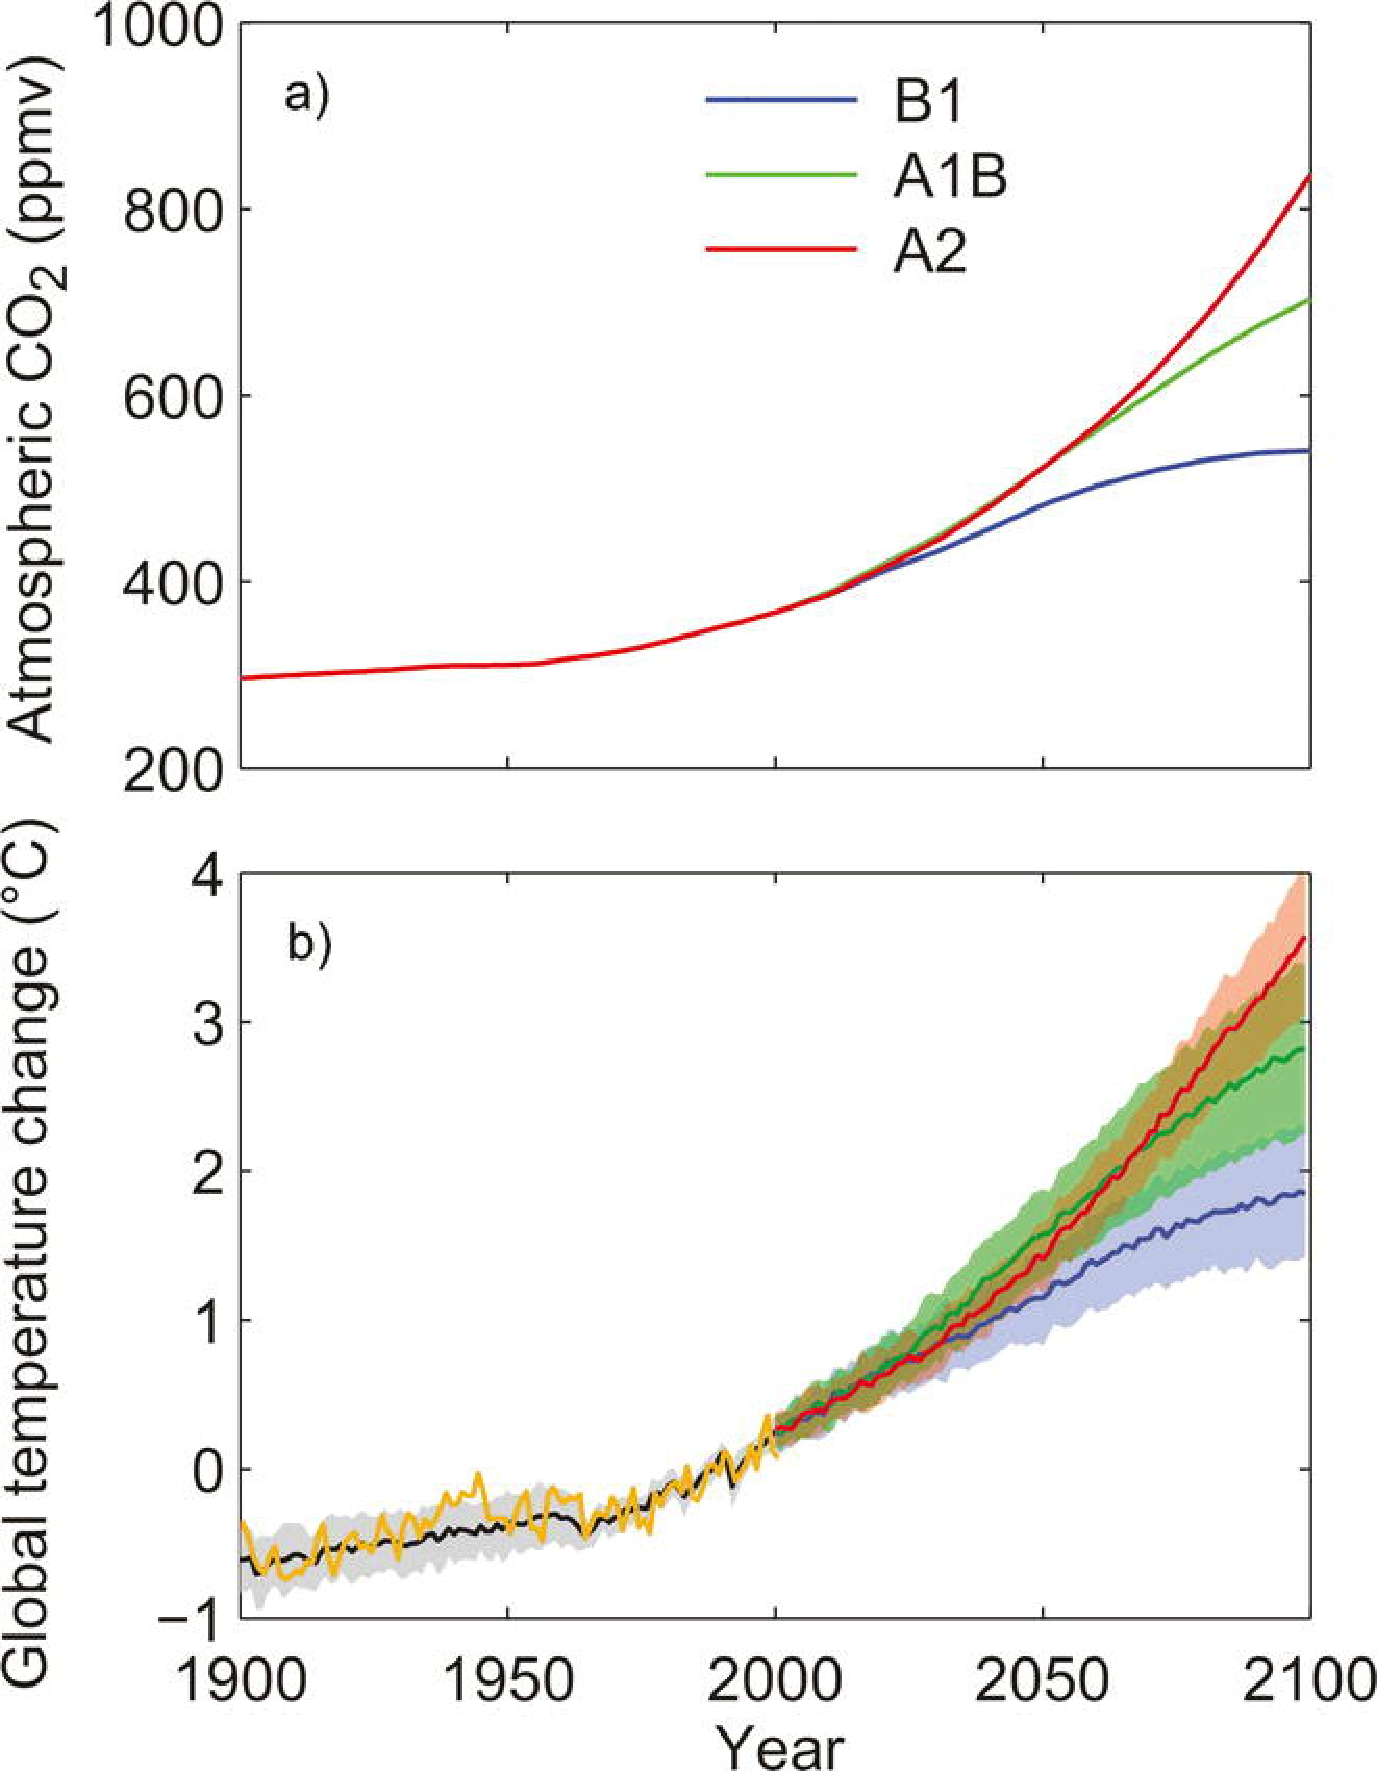
\includegraphics[width=19pc,angle=0]{figure01.pdf}\\
%  \caption{Enter the caption for your figure here.  Repeat as
%  necessary for each of your figures. Figure from \protect\cite{Knutti2008}.}\label{f1}
%\end{figure}

% NOTE: what to include in the paper, key questions.
% The paper should provide insight about what might happen if a large volcano erupted
% (order of magnitude or more than Mt.\ Pinatubo). How does the atmosphere react, for
% example in the aerosol dynamics? (QBO, SO2/AOD/RF relationship.) It should also be
% about how volcanic simulations compare in magnitude and if there is time for more
% simulations, how model complexity (dynamic ocean against slab ocean) affect things.
% - How far does the linear relation between AOD and RF go? What phases does the
%   aerosols go though? (Perhaps the most promising avenue.)
% - How much does it matter how high in the atmosphere the initial SO2 is injected?
%   (Already is some literature on this, suggesting it is not much. Also some on
%   latitude dependence, which has a bigger influence.)
% - How does the climate response change based on the state of the climate: what if we
%   run a CO2 doubling or quadrupling simulation until close to equilibrium, and let the
%   volcanoes erupt then? (Lack the doubling scenario, and setting it up has resulted in
%   strange output that must be resolved. Could take a while.)

\section{Introduction}

% NOTE: Suggested layout for the introduction
% - The objectives of the work.
% - The justification for these objectives: Why is the work important?
% - Background: Who else has done what? How? What have we done previously?
% - Guidance to the reader: What should the reader watch for in the paper? What are the
%   interesting high points? What strategy did we use?
% - Summary/conclusion: What should the reader expect as conclusion? In advanced
%   versions of the outline, you should also include all the sections that will go in
%   the Experimental section (at the level of paragraph subheadings) and indicate what
%   information will go.

% Toohey et al 2011 have a nice end of introduction.

\Gls{rf} and \gls{aod} are crucial metrics representing the energy imbalance at
\gls{toa} and the stratospheric opacity due to aerosol scattering, respectively. They
are extensively used to quantify the impact of major volcanic eruptions. The assumption
of a linear dependency of \gls{rf} on \gls{aod} is commonly adopted
\citep{myhre2013,andersson2015}, and applying such a linear relationship has yielded
reasonably accurate estimates in climate model simulations of volcanic eruptions
\citep{mills2017,hansen2005,gregory2016,marshall2020,pitari2016b}. Yet, a wide spread in
the estimated aerosol forcing efficiencies (\gls{rf} normalised by \gls{aod}) exists
among studies, spanning approximately from \(\sim
\SI{-15}{\watt\metre^{-2}\ce{AOD}^{-1}}\) \citep{pitari2016b} to \(\sim
\SI{-25}{\watt\metre^{-2}\ce{AOD}^{-1}}\) \citep{myhre2013}. Additionally, these
estimates are predominantly based on small eruptions with \gls{aod} values up to at most
\(\sim 0.7\).

Although \ce{H2O}, \ce{N2}, and \ce{CO2} are the most abundant gases emitted by
volcanoes \citep{robock2000}, sulphur species such as \ce{SO2} provide a greater
influence due to the comparatively high background concentrations of the former gases in
the atmosphere. The transformation of \ce{SO2} molecules through reactions with \ce{OH}
and \ce{H2O} leads to the formation of sulphuric acid (\ce{H2SO4}) \citep{robock2000},
which scatters sunlight thereby elevating planetary albedo and reducing the \gls{rf}. As
the conversion from \ce{SO2} to \ce{H2SO4} occurs over weeks \citep{robock2000}, the
peak \gls{rf} experiences a slight delay from the eruption's peak \ce{SO2} injection.
The lifetime of the \ce{H2SO4} aerosols in the stratosphere depends on various factors,
including latitude \citep{marshall2019, toohey2019}, volcanic plume height
\citep{marshall2019}, aerosol size \citep{marshall2019}, the quasi-biennial oscillation
phase \citep{pitari2016b} and the season of the year (determining to which hemisphere
aerosols are transported) \citep{toohey2011,toohey2019}. In the case of tropical
eruptions, aerosols are typically transported poleward in the stratosphere and descend
back to mid-latitude troposphere within one to two years \citep{robock2000}. Upon
descending below the tropopause, these aerosols are readily removed by wet deposition
\citep{liu2012}.

Before the current era of significant anthropogenic climate forcing, volcanic eruptions
were the primary forcing mechanism dictating Earth's climate variability during the
Holocene period \citep{sigl2022}. Despite this substantial impact, few climate-model
experiments have included volcanic forcing when simulating climate evolution during the
Holocene \citep{sigl2022}, likely implying an exaggerated positive forcing
\citep{gregory2016,solomon2011}. This absence of persistent cooling is one of several
factors that have been suggested to contribute to the common disparity between simulated
and observed global warming \citep{andersson2015}. Despite extensive attention on
understanding the way volcanic eruptions influence climate, questions regarding aerosol
particle processes---such as growth and creation rates when \ce{OH} is scarce---remain
unanswered \citep[e.g.~][]{robock2000,zanchettin2019,marshall2020,marshall2022}. These
processes impact aerosol scattering efficiency and potentially the \gls{rf} to \gls{aod}
relationship. \citet{marshall2020} observe higher aerosol forcing efficiency in
post-eruption years \(2\) and \(3\) compared to year 1, and attribute this post-eruption
increase in aerosol forcing efficiency to strong spatial concentration in the initial
year and subsequent distribution of aerosols over a larger area. This spatial
redistribution increases the albedo per global mean \gls{aod} thereby causing a stronger
\gls{rf} to \gls{aod} ratio \citep{marshall2020}.

Previous studies of both Mt.\ Pinatubo \citep{mills2017,hansen2005} and volcanoes within
the instrumental era \citep{gregory2016} have been used to estimate the relationship
between the \gls{rf} energy imbalance and change in \gls{aod} caused by volcanic
eruptions. While \citet{myhre2013} employ a formula scaling \gls{rf} by \gls{aod} to
obtain \(\SI{-25}{\watt\metre^{-2}\mathrm{AOD}^{-1}}\), recent literature reports
estimates down to \(\SI{-19.0(5)}{\watt\metre^{-2}\mathrm{AOD}^{-1}}\)
\citep{gregory2016} and \(\SI{-18.3(10)}{\watt\metre^{-2}\mathrm{AOD}^{-1}}\)
\citep{mills2017}. Synthetic volcano simulations in \citet{marshall2020} yield a scaling
factor of \(\SI{-20.5(2)}{\watt\metre^{-2}\mathrm{AOD}^{-1}}\) across an ensemble of
\(82\) simulations featuring varying injection heights and latitudes of volcanic
emissions, with \iso{} ranging from \(10\) to \(\SI{100}{\tera\gram(\ce{SO2})}\).

A similar simulation setup, albeit with notable differences, was conducted by
\citet{niemeier2015}, involving an ensemble of \(14\) levels of injected sulphur
spanning between \(\SI{1}{\tera\gram(\ce{S})\mathrm{yr}^{-1}}\)
(\(\SI{2}{\tera\gram(\ce{SO2})\mathrm{yr}^{-1}}\)) and
\(\SI{100}{\tera\gram(\ce{S})\mathrm{yr}^{-1}}\)
(\(\SI{200}{\tera\gram(\ce{SO2})\mathrm{yr}^{-1}}\)). These geoengineering simulations
maintained continuous sulphur injections, running until a steady sulphur level was
achieved. Results indicated an inverse exponential relationship between \gls{rf} and
\iso{} rate, converging to \(\SI{-65}{\watt\metre^{-2}}\)
(Eq.~\ref{eq:niemeier_exponential}). Even the \(100\times\) Mt.\ Pinatubo super-volcano
simulation by \citet{jones2005}, which obtained a peak \gls{rf} of
\(\SI{-60}{\watt\metre^{-2}}\), is below the suggested limit of
\(\SI{-65}{\watt\metre^{-2}}\). Moreover, \citet{timmreck2010} find a peak \gls{rf}
anomaly of \(\SI{-18}{\watt\metre^{-2}}\) from a \(\SI{1700}{\tera\gram(\ce{SO2})}\)
eruption simulation, which corresponds well with the function estimated by
\citet{niemeier2015} at the given \ce{SO2} level. Several studies have demonstrated a
linear relationship of approximately \(-\SI{20}{\watt\metre^{-2}\mathrm{AOD}^{-1}}\)
between \gls{rf} and \gls{aod}, although substantial variability exists in the slope
among studies \citep{mills2017,hansen2005,gregory2016,marshall2020,pitari2016b}.
Moreover, a time-after-eruption dependence on the \gls{rf} to \gls{aod} ratio is found
in \citet{marshall2020}, whereas \citet{niemeier2015} revealed a non-linear relationship
between \gls{rf} and \iso{} rate. Thus, a consensus on the relationship between \iso{},
\gls{aod}, and \gls{rf} has yet to be established.

One avenue that has garnered considerable attention is comparing the magnitude of
volcanic or volcano-like forcings to increased \ce{CO2} levels. Several studies explore
the connection between volcanic forcing and the climate sensitivity to a doubling of
\ce{CO2}
\citep{boer2007,marvel2016,merlis2014,ollila2016,richardson2019,salvi2022,wigley2005}.
The comparison of forcing from volcanoes and \ce{CO2} aims to mitigate the large
uncertainty in estimates of the sensitivity of the real climate system. Inferring
climate sensitivity from volcanic eruption events has been attempted as a way to
constrain the sensitivity \citep{boer2007} by assuming that volcanic and \ce{CO2}
forcings produce similar feedbacks \citep{pauling2023}. Earlier studies suggest the
potential for constraining \gls{ecs} using volcanoes \citep{bender2010}, provided that
\gls{ecs} is constrained by \gls{erf} rather than \gls{irf}, as \gls{erf} accounts for
rapid atmospheric adjustments in contrast to \gls{irf} \citep{richardson2019}. However,
other studies refute this approach, pointing out that different sensitivities of
volcanic forcing and \ce{CO2} doubling seem to exist \citep{douglass2006}, or that
constraining the \gls{ecs} by \gls{erf} lacks accuracy due to the precision of climate
simulations \citep{boer2007,salvi2022}. Although \gls{erf} offers a more suitable
indicator of forcing than \gls{irf} \citep{marvel2016,richardson2019}, more recent
studies conclude that \gls{ecs} cannot be constrained from volcanic eruption events
\citep{pauling2023}.

Employing eruptions in the medium to super-volcano size enhances the signal-to-noise
ratio without necessitating an extensive and computationally expensive ensemble, and as
such, is a tempting way to mimic a large ensemble of smaller volcanic eruptions.
However, the \gls{aod}, \gls{rf}, and temperature signatures are not guaranteed to be a
simple scaling of that of smaller volcanic eruptions. Previous studies have simulated
super-volcanoes using \gls{aod} as the input forcing, where the \gls{aod} was that of
Mt.\ Pinatubo scaled by one hundred \citep{jones2005}. This approach may yield incorrect
results, both because the peak of the \gls{aod} may be too small or big, but also
because the evolution of the \gls{aod} could be inappropriate. Likewise, a different
\gls{aod} evolution may be found from similar size eruptions, but at different
latitudes. To investigate this issue, our simulations are based on \iso{} covering three
orders of magnitude.

We conducted ensemble simulations of volcanic eruptions in the \gls{cesm2} coupled with
the \gls{waccm}. The ensembles span \iso{} levels of three orders of magnitude with four
members for each: \(\SI{26}{\tera\gram(\ce{SO2})}\), \(\SI{400}{\tera\gram(\ce{SO2})}\),
and \(\SI{1629}{\tera\gram(\ce{SO2})}\). Details regarding the experimental setup are
provided in section~\ref{sec:method}. Our findings reveal non-linear \gls{rf} to
\gls{aod} dependencies for medium to super-volcano size eruptions. Additionally, we
observe a time-dependent variation in the \gls{rf} to \gls{aod} ratio, detailed in
section~\ref{sec:results} and discussed in section~\ref{sec:discussion}. Furthermore,
our data, along with insights from previous studies, suggest that the \gls{rf}
dependency on \iso{} identified by \citet{niemeier2015} acts as a lower boundary. Our
conclusions are presented in section~\ref{sec:conclusions}.

\section{Method}\label{sec:method}

\subsection{Model}

We use the \gls{cesm2} \citep{danabasoglu2020} in conjunction with the \gls{waccm}
\citep{gettleman2019} and the fully dynamical ocean component \gls{pop}
\citep{smith2010, danabasoglu2020}. The atmosphere model was run at a nominal
\(\SI{2}{\degree}\) resolution with \(70\) vertical levels in the \gls{ma}
configuration.

The \gls{waccm} version employed in the \gls{ma} configuration uses the \gls{mam3}
\citep{gettleman2019}, a simplified and computationally efficient default setting within
the \gls{cam5} \citep{liu2016}, as described in \citet{liu2012}. The \gls{mam3} was
developed from MAM7 and features the modes Aitken, accumulation, and coarse
\citep{liu2016}.

\subsection{Simulations}

Appendix A provides a description of the simulation setup and utilised output variables.
Table~\ref{tab:simulation-overview} summarises the simulations, encompassing three
\ce{SO2} injection magnitudes across four seasons: 15 February, 15 May, 15 August, and
15 November. The magnitudes vary over three orders of magnitude:
\(\SI{26}{\tera\gram(\ce{SO2})}\), \(\SI{400}{\tera\gram(\ce{SO2})}\), and
\(\SI{1629}{\tera\gram(\ce{SO2})}\).

The smallest eruption case, \gls{c2wm}, is similar in magnitude as compared to events
like Mt.\ Pinatubo
\citep[\(\sim10\)--\(\SI{20}{\tera\gram(\ce{SO2})}\);][]{timmreck2018} and Mt.\ Tambora
\citep[\(\sim\SI{56.2}{\tera\gram(\ce{SO2})}\);][]{zanchettin2016}. The intermediate
case, \gls{c2wmp}, resembles the magnitude of the Samalas eruption in 1257
\citep[\(\sim{144}\)--\(\SI{170}{\tera\gram(\ce{SO2})}\);][]{vidal2016}, while the
largest eruption case, \gls{c2ws}, is in the likely range of the \gls{ytt} eruption
occurring about \(\SI{72000}{\mathrm{yr}}\) ago
\citep[\(100\)--\(\SI{10000}{\tera\gram(\ce{SO2})}\);][]{jones2005}. All eruptions were
situated at the equator (\(\SI{0}{\degree N}\), \(\SI{1}{\degree E}\)) with \ce{SO2}
injected between \(\SI{18}{\kilo\meter}\) and \(\SI{20}{\kilo\meter}\) altitude.
Collectively, the three eruption cases \gls{c2wm}, \gls{c2wmp}, and \gls{c2ws} are
referred to as \gls{c2w}. Two additional high-latitude eruptions, labelled \gls{c2wsn},
of the same \iso{} magnitude as \gls{c2ws} were simulated at \(\SI{56}{\degree N}\),
\(\SI{287.7}{\degree E}\) with a six-month separation (15 February and 15 August).

\begin{table*}
  \centering

  \caption{\gls{cesm2} simulations. The ensembles \gls{c2wsn} and \gls{c2ws} have the same
    eruption magnitude, but while \gls{c2ws} is located at the equator, \gls{c2wsn} is
    located at a high northern latitude. \gls{c2wmp} and \gls{c2wm} are located at the
    equator, but with different magnitudes compared to \gls{c2ws}. All tropical ensembles
    have four members, indicated by the number of eruption months, while the northern
    latitude ensemble consists of two members.}\label{tab:simulation-overview}%
  \begin{center}
    \begin{tabular}[c]{cccccc}
      Ensemble name                   & \(\si{\tera\gram(\ce{SO2})}\)         &
      Lat [\si{\degree\mathrm{N}}]    & Lon [\si{\degree\mathrm{E}}]          & Alt [\si{\kilo\metre}] & Eruption months \\
      \gls{c2wsn}                     & \(1629\)                              &
      \(56\)                          & \(287.7\)                             &
      \(18\)--\(20\)                  & Feb,\hphantom{May,}Aug\hphantom{,Nov}                                            \\
      \gls{c2ws}                      & \(1629\)                              &
      \(\hphantom{1}0\)               & \(\hphantom{28}1\hphantom{.7}\)       & \(18\)--\(20\)
                                      & Feb,May,Aug,Nov                                                                  \\
      \gls{c2wmp}                     & \(\hphantom{1}400\)                   &
      \(\hphantom{1}0\)               &
      \(\hphantom{28}1\hphantom{.7}\) &
      \(18\)--\(20\)                  & Feb,May,Aug,Nov                                                                  \\
      \gls{c2wm}                      & \(\hphantom{14}26\)                   &
      \(\hphantom{1}0\)               &
      \(\hphantom{28}1\hphantom{.7}\) & \(18\)--\(20\)
                                      & Feb,May,Aug,Nov                                                                  \\
    \end{tabular}
  \end{center}
\end{table*}

\section{Results}\label{sec:results}

% NOTE: the results should be laid out in a logical way, with the most
% interesting/important stuff first, then tangents that dig deeper at specific things
% later.
% 1. RF to AOD time-after-eruption dependence should be top priority
% 2. Then probably temperature scaling since we discuss the shape of both AOD and RF
%    time series before that (MOTIVATION: can we expect a specific temperature time
%    series shape based on the shape of either of or both of the RF and AOD time
%    series?)
% 3. If there is something interesting to say about the rest of the figures (all the
%    comparing of parameters), then this should come here.

\subsection{Analysis of the time series}

Figure~\ref{fig:1_compare_waveform} presents time series of global mean \gls{aod},
\gls{rf}, and surface air temperature. The black lines represent the medians across the
four-member ensembles, while shading indicates the 5th to 95th percentiles. The three
distinct forcing magnitudes (\gls{c2wm}, \gls{c2wmp}, and \gls{c2ws}) outlined in
table~\ref{tab:simulation-overview} have been used. The time series in
Fig.~\ref{fig:1_compare_waveform} are normalised by setting the peak value to unity,
defined based on the peak of a fit from a Savitzky-Golay filter of 3rd order and a
one-year window length \citep{savitzky1964}.

% NOTAT:
% Jeg forstår ikke dette argumentet - hvis RF er lik for alle, hvordan kan temperaturen (som er forskjellig mellom dem) være avhenging av RF?
A notable feature across the subfigures of Fig.~\ref{fig:1_compare_waveform} is the peak
occurrence of the \gls{c2wm} case compared to the larger eruption cases. The peak of
\gls{c2wm} arrives earlier for both \gls{aod} (Fig.~\ref{fig:1_compare_waveform}a) and
temperature (Fig.~\ref{fig:1_compare_waveform}c), while the \gls{rf} time series in
Fig.~\ref{fig:1_compare_waveform}b are all indistinguishable. Cases \gls{c2wmp} and
\gls{c2ws} are indistinguishable in their temperature development, and while \gls{c2wm}
peaks at an earlier time, it decays similarly to the other two cases. Interestingly, the
same development between \gls{c2wmp} and \gls{c2ws} is not found in the \gls{aod} time
series. \gls{c2wm} peaks at an earlier time, but also spends more time around the peak
and as such decays at a later time post-eruption. Likewise, \gls{c2wmp} has a faster
rise and slower decay compared to \gls{c2ws}, but where both peak at a similar time.

The timescale of the perturbation of \gls{aod} and \gls{rf} is shorter than that of the
temperature. While the \gls{aod} and \gls{rf} time series return to their equilibrium
state within roughly three years, the temperature time series remain heavily perturbed
three years post-eruption. Even when running the simulations for 20 years post-eruption,
the temperature time series are still decaying.

\begin{figure}
  \centering
  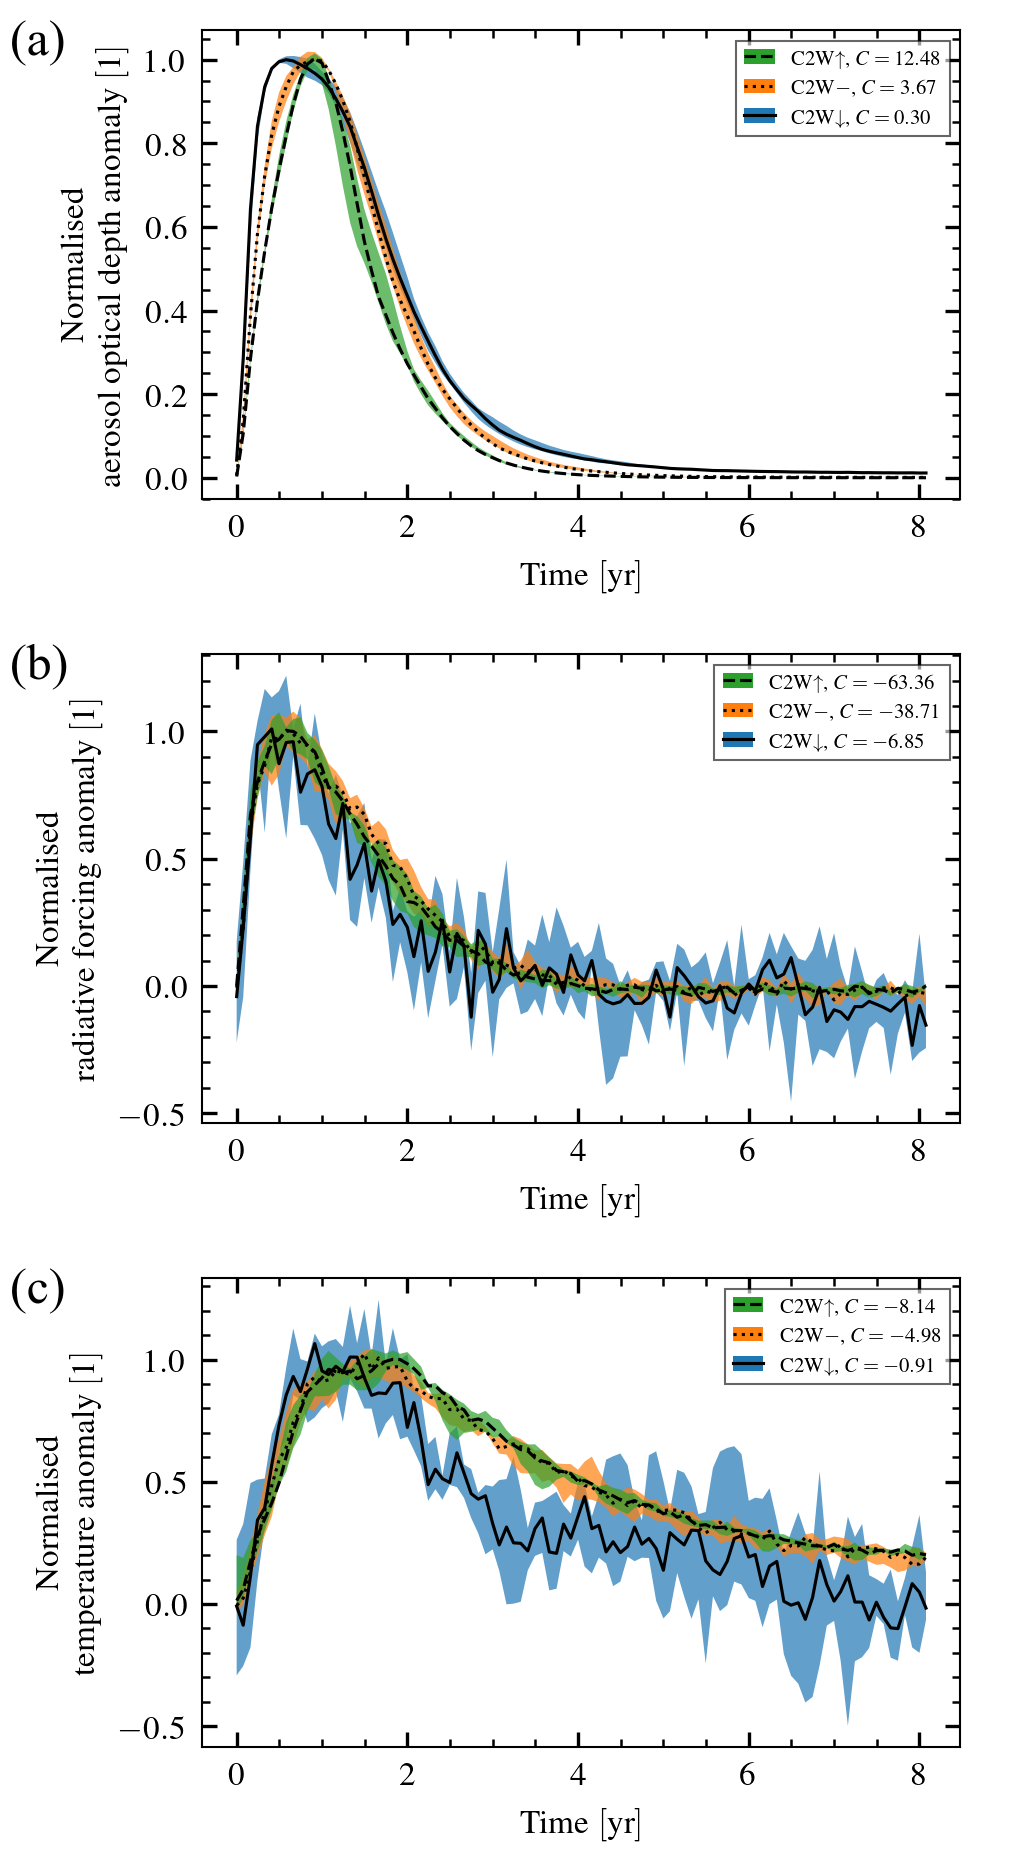
\includegraphics[width=0.5\linewidth]{figures/figure1.png}

  \caption{\gls{aod} (a), \gls{rf} (b) and temperature response (c) time series to the
    three tropical volcanic eruption cases, \gls{c2wm}, \gls{c2wmp} and \gls{c2ws}. The time
    series have been normalised to have peak values at unity, where \(C\) is the
    normalisation constant. Black lines indicate the median across the four-member
    ensembles, while shading marks the 5th and 95th
    percentiles.}\label{fig:1_compare_waveform}%
\end{figure}

\subsection{\gls{rf} dependency on \gls{aod}}

We next focus on the development of the \gls{aod} and \gls{rf} time series relative to
each other. Similar comparisons were conducted in \citet[][their Fig.\ 4]{gregory2016}
and \citet[][their Fig.\ 1]{marshall2020}, with \gls{rf} plotted against \gls{aod}.
Figure~\ref{fig:2_rf_vs_aod_slopes} displays annual mean values from the four simulation
cases in table~\ref{tab:simulation-overview}; the small eruption case (\gls{c2wm}) as
blue downward-pointing triangles, the intermediate eruption case (\gls{c2wmp}) as orange
thick diamonds, the large tropical eruption case (\gls{c2ws}) as green upward-pointing
triangles, and the large northern hemisphere eruption case (\gls{c2wsn}) as brown
upward-pointing three-branched twigs. Also shown are the data from \citet[][Fig.\ 4,
  black crosses from HadCM3 sstPiHistVol]{gregory2016} as grey crosses labelled \gls{g16}
(described in Appendix B, section~\ref{ap:g16}). Additionally, the estimated peak values
from the Mt.\ Pinatubo and Mt.\ Tambora eruptions are plotted as a black star and plus,
while the peak from the \citet{jones2005} simulation is shown as a pink square labelled
\gls{j05}. Finally, red circles represent the peak values obtained from the \gls{c2w}
tropical eruption cases. The straight lines are the same as shown by
\citet{gregory2016}. The full data range is shown in Fig.~\ref{fig:2_rf_vs_aod_slopes}a
while Fig.~\ref{fig:2_rf_vs_aod_slopes}b highlights a narrow range, focusing on the
\gls{c2wm} case.

The annual mean data from the Pinatubo-like \gls{c2wm} case in
Fig.~\ref{fig:2_rf_vs_aod_slopes}b have \gls{rf} values as a function of \gls{aod} that
follow almost the same constant slope as the \gls{g16} data. However, in
Fig.~\ref{fig:2_rf_vs_aod_slopes}a we observe that the stronger eruptions lead to
dissimilar responses in \gls{aod} and \gls{rf}, where \gls{c2wmp} seems to follow close
to a \(-10\) slope and \gls{c2ws} is closer to a \(-5\) slope.
% NOTAT:
% Dette kan komme tydeligere fram i diskusjon og konklusjon, bare pass på at det ikke går imot det du sier om fig. 3
The peak values (red circles) suggest a non-linear dependence, while within each
eruption strength (same colour) the annual mean values fall relatively close to a
straight line.

\begin{figure}
  \centering
  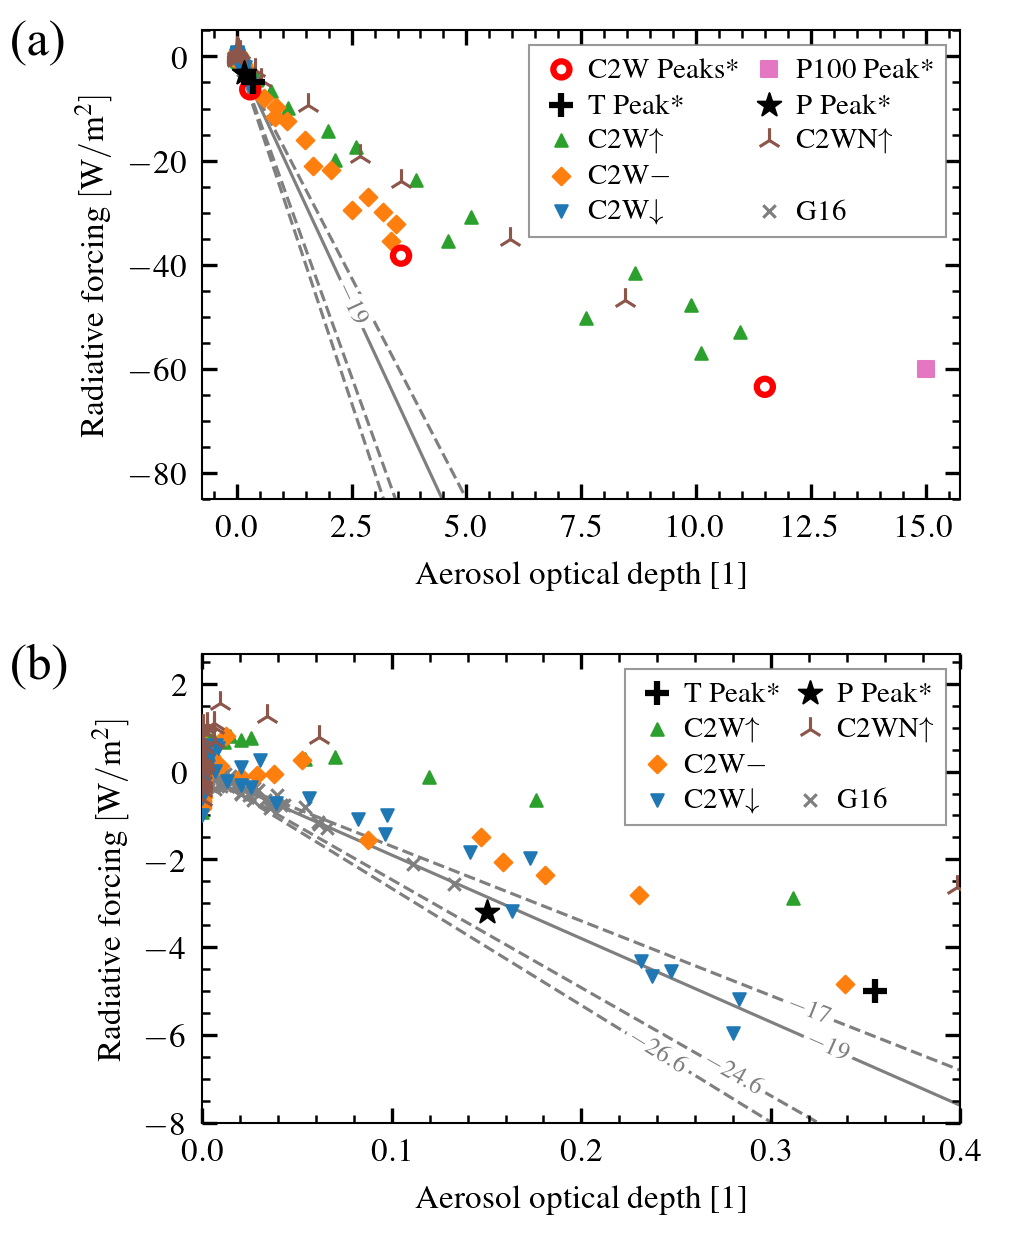
\includegraphics[width=0.5\linewidth]{figures/figure2.png}

  \caption{\gls{rf} as a function of \gls{aod}, yearly means. Data from the four
    simulations listed in table~\ref{tab:simulation-overview} (\gls{c2wm}, \gls{c2wmp},
    \gls{c2ws} and \gls{c2wsn}) are shown along with the data from the HadCM3 sstPiHistVol
    simulation by \citet{gregory2016} (grey crosses, \gls{g16}). Also shown are the
    estimated peak values of the Mt.\ Pinatubo (black star) and Mt.\ Tambora (black plus)
    eruptions. The peak values from the simulations \gls{c2wm}, \gls{c2wmp} and \gls{c2ws}
    are shown as red circles. Additionally in (a) the simulated super-volcano of
    \citet{jones2005} (pink square) is shown. All peak values (as opposed to annual means)
    have an asterisk (\(\ast{}\)) in their label. The grey lines are the same regression
    fits as in \citet[][Fig.\ 4]{gregory2016}, where the solid line is the fit to \gls{g16}.
    (b): Zooming in on the smallest \gls{aod} values.}\label{fig:2_rf_vs_aod_slopes}%
\end{figure}

To investigate the time dependence of the ratio between \gls{rf} and \gls{aod}, we
present seasonal means of this ratio in Fig.~\ref{fig:3_rf_to_aod_ratios}, where the
start of the time series is taken as the eruption day. The plot shows all the eruption
cases given in table~\ref{tab:simulation-overview}, as well as the tropical eruptions
from \citet{marshall2020dataset} (\(6\) of \(82\) eruptions), labelled \gls{m20} and
described in Appendix B, section~\ref{ap:m20}. In Fig.~\ref{fig:3_rf_to_aod_ratios}a,
lines are linear regression fits to the seasonal means across all ensemble members,
summarised in table~\ref{tab:slope-gradients}. Shaded regions are the standard deviation
around the seasonal means. A similar shading is plotted in
Fig.~\ref{fig:3_rf_to_aod_ratios}b, but where the regression fits have been omitted for
clarity. As the \gls{aod} and \gls{rf} time series start from zero, the ratio from the
first season is not included. Likewise, after three years both time series are almost
fully equilibrated (Fig.~\ref{fig:1_compare_waveform}a,b). The data is further divided
into two periods; a pre-peak period where the peak of both the \gls{aod} and the
\gls{rf} is included (consisting of the first post-eruption year), and a post-peak
period for the decaying part (consisting of the second and third post-eruption years).

% NOTAT:
% Hva er første og andre periode og hvorfor har du valgt den indelingen? Før og etter peak (isåfall: pre-peak og post-peak)?
Although the ratio changes across the eruption magnitudes, we find that all the tropical
cases follow a positive slope during the pre-peak period, as seen in
Fig.~\ref{fig:3_rf_to_aod_ratios}a and described in table~\ref{tab:slope-gradients}. The
northern latitude case in \gls{c2wsn} shows a much flatter slope compared to \gls{c2w}
and \gls{m20}. The distinction between the slopes from the tropical and non-tropical
cases is perhaps more clear in Fig.~\ref{fig:3_rf_to_aod_ratios}b and corresponding rows
in table~\ref{tab:slope-gradients}. Again, \gls{c2wsn} shows an almost flat slope
compared to the tropical cases. During the second period, more noise is introduced, but
a weak tendency of negative slopes is found among the tropical cases, as well as in the
\gls{c2wsn} case up to the last season where the noise is also the largest.

\begin{table}
  \centering

  \caption{Slope and standard deviation for the data in Fig.~\ref{fig:3_rf_to_aod_ratios}.
    The regression fits in the top half of the table are for
    Fig.~\ref{fig:3_rf_to_aod_ratios}a, while the bottom half is for
    Fig.~\ref{fig:3_rf_to_aod_ratios}b. The columns ``pre-peak'' and ``post-peak'' refer to
    the two periods as shown in Fig.~\ref{fig:3_rf_to_aod_ratios}. The ensembles are the
    same as those given in table~\ref{tab:simulation-overview}, in addition to the \(6\)
    tropical eruptions from the \(82\) member ensemble in
    \citet{marshall2020}.}\label{tab:slope-gradients}%
  \begin{tabular}{cccc}
    Figure                                          & Ensemble name & Pre-peak        & Post-peak        \\
    \rowcolor{LightGray}                            & \gls{c2wsn}   & \(0.45\pm1.15\) & \(1.51\pm1.45\)  \\
    \rowcolor{LightGray}                            & \gls{c2ws}    & \(3.85\pm0.52\) & \(-3.29\pm0.60\) \\
    \rowcolor{LightGray}                            & \gls{c2wmp}   & \(4.36\pm0.82\) & \(-3.37\pm0.59\) \\
    \rowcolor{LightGray}                            & \gls{c2wm}    & \(3.64\pm2.41\) & \(-1.41\pm3.25\) \\
    \rowcolor{LightGray}                            & \gls{m20}     & \(6.34\pm1.77\) & \(-0.36\pm1.33\) \\
    \multirow{5}{*}{\ref{fig:3_rf_to_aod_ratios}b}  & \gls{c2wsn}   & \(0.08\pm0.20\) & \(0.27\pm0.26\)  \\
    \multirow{-9}{*}{\ref{fig:3_rf_to_aod_ratios}a} & \gls{c2ws}    & \(0.75\pm0.10\) & \(-0.64\pm0.12\) \\
                                                    & \gls{c2wmp}   & \(0.43\pm0.08\) & \(-0.34\pm0.06\) \\
                                                    & \gls{c2wm}    & \(0.18\pm0.12\) & \(-0.07\pm0.16\) \\
                                                    & \gls{m20}     & \(0.33\pm0.07\) & \(-0.02\pm0.08\) \\
  \end{tabular}
\end{table}

% NOTAT:
% Her bør du vurdere å splitte opp klarere mellom første periode og andre peroide - og bruk samme begrep som over, om mulig
\citet[][their Fig.\ 1c,d]{marshall2020} present results that demonstrate a
time-dependent relationship in the conversion between \gls{aod} and \gls{rf}. They
obtain an \gls{rf} to \gls{aod} ratio with a negative slope when comparing the first
post-eruption year to the second and third. As such, \citet{marshall2020} find that, on
average, the aerosol forcing efficiency increases during the first two to three
post-eruption years. This phenomenon is explained by \citet{marshall2020} as the
aerosols initially being spatially confined to the hemisphere where the eruption
occurred. Subsequently, during the second and third years, they spread globally,
resulting in a higher global-mean albedo per \gls{aod} and consequently a stronger
\gls{rf} per \gls{aod} ratio with time. However, as noted above, a decrease in aerosol
forcing efficiency is found when analysing the \gls{m20} data with seasonal resolution
during the pre-peak period (first year post-eruption) while constraining the ensemble to
only include eruptions within \(-10\) to \(\SI{10}{\degree\mathrm{N}}\). The post-peak
period shows an increasing aerosol forcing efficiency, and during the full first three
post-eruption years (pre-peak and post-peak), both the tropical subset and the full
\gls{m20} data yield an increasing efficiency. Likewise, the first three post-eruption
years of the \gls{c2wmp}, \gls{c2ws}, and \gls{c2wsn} cases show a weak negative slope
and thus an increasing efficiency, while \gls{c2wm} shows an elevated post-peak ratio as
seen in Fig.~\ref{fig:3_rf_to_aod_ratios}b.

We also note that while the aerosol forcing efficiency is decreasing for tropical
\gls{m20} data in the pre-peak period, the full dataset shows increasing efficiency.
This is in line with what we find from \gls{c2wsn}, which is the only eruption case that
does not show a clear aerosol forcing efficiency decrease during the pre-peak period.

\begin{figure}
  \centering
  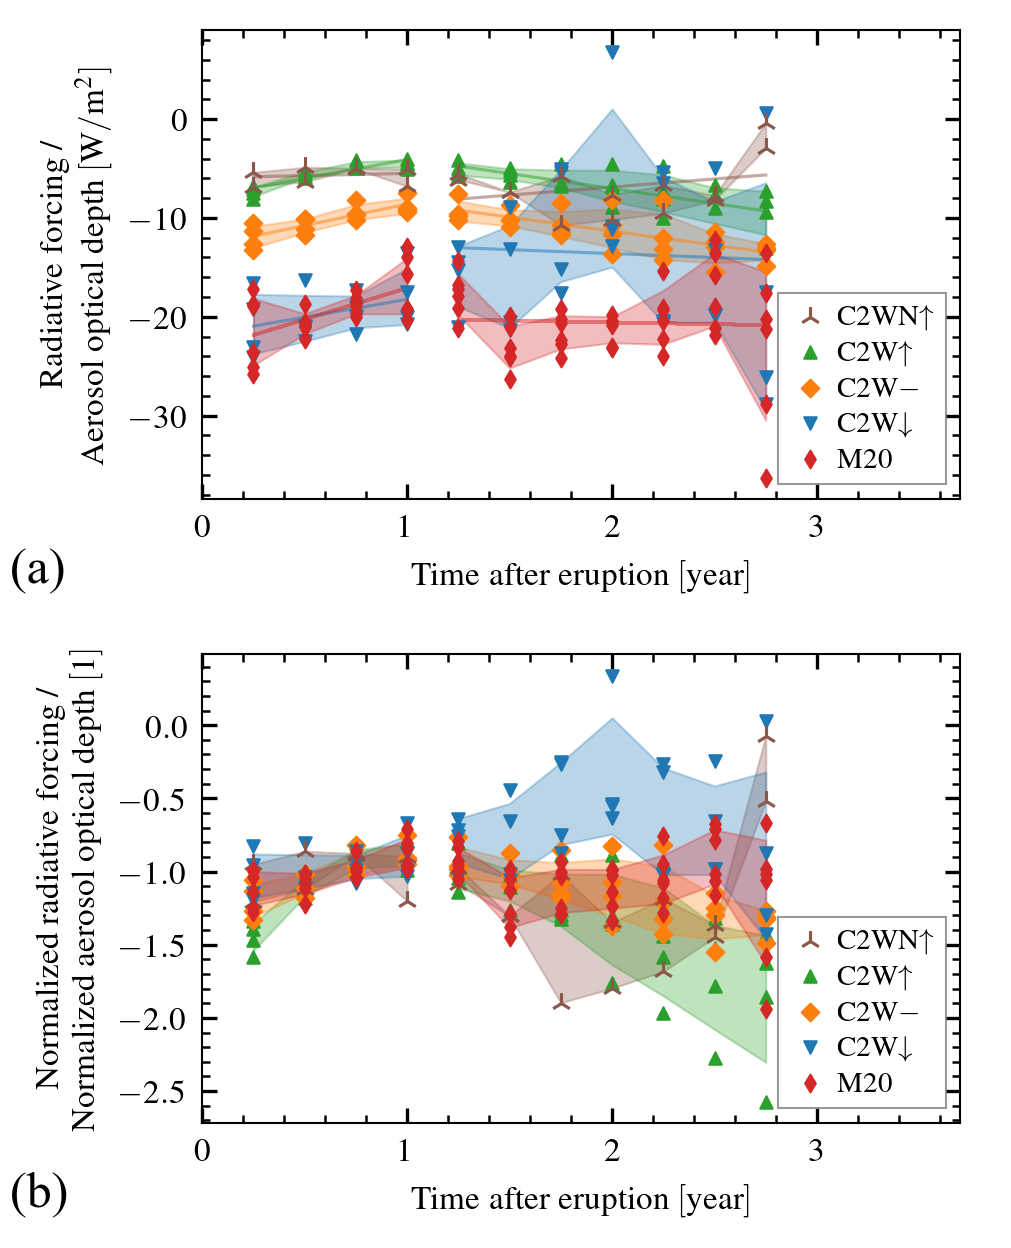
\includegraphics[width=0.5\linewidth]{figures/figure3.png}

  \caption{(a): The ratio of \gls{rf} to \gls{aod}, with time-after-eruption on the
    horizontal axis. Straight lines indicate linear regression fits and are described in
    table~\ref{tab:slope-gradients}, while shaded regions are the standard deviation across
    the ensembles for each season. Regression fits and shadings are made for the pre-peak
    and post-peak periods. (b): Same as in (a), but where the underlying \gls{aod} and
    \gls{rf} time series have been scaled to have peak values at unity. Shown are data from
    table~\ref{tab:simulation-overview} along with tropical eruptions from
    \gls{m20}.}\label{fig:3_rf_to_aod_ratios}%
\end{figure}

\subsection{Parameter scan}

% NOTAT:
% Gå heller gjennom hver figur for seg først, så tar du dette på slutten med diagrammet vi snakket om.
In Fig.~\ref{fig:4_parameter_scan}, we compare the peak values of all investigated
\gls{cesm2} output parameters against each other as well as to \iso{}. For our tropical
cases (\gls{c2w}), we observe in Fig.~\ref{fig:4_parameter_scan}a an almost linear
relationship between \gls{aod} peak values and \iso{}. The latitude also plays a role in
the magnitude of the \gls{aod} perturbation, evident from \gls{c2wsn}. This weak yet
notable latitude dependence aligns with findings by \citet{marshall2019}, indicating
that \(\SI{72}{\percent}\) of the \gls{aod} variance can be attributed to \iso{}, while
latitude accounts for only \(\SI{16}{\percent}\) of the variance. Peak values from their
data (82 simulations) plotted as red thin diamonds display a similar pattern, with
\gls{aod} exhibiting close to linear dependence on \iso{}, but with latitude introducing
a spread in \gls{aod}. Peak values from Mt.\ Pinatubo (P) and Mt.\ Tambora (T) are shown
for reference, along with peak values from \citet{jones2005} labelled \gls{j05} and
\citet{timmreck2010} labelled \gls{t10}. The \gls{j05} is a simulation of a
super-volcano based on a \(100\) times scaling of the \gls{aod} from Mt.\ Pinatubo,
while \gls{t10} is a simulation of the \gls{ytt} eruption based on \ce{SO2} injections.

In Fig.~\ref{fig:4_parameter_scan}b, \gls{rf} plotted against \iso{} (with the absolute
value of \gls{rf} on the \(y\)-axis) indicates a substantial damping effect on \gls{rf}
as \iso{} increases for the \gls{c2w} data, in agreement with results from
\citet{ottobliesner2016}, labelled \gls{ob16}. The \gls{ob16} data come from a \(2500\)
year long simulation using historic volcanoes as the only external forcing. The analysis
details of \gls{ob16} can be found in Appendix B, section~\ref{ap:ob16}. Despite the
model complexity difference, \citet{ottobliesner2016}'s simulations using \gls{cesm1}
with a low-top atmosphere (\gls{cam5}) produce \glspl{rf} comparable to our findings.

\begin{figure*}
  \centering
  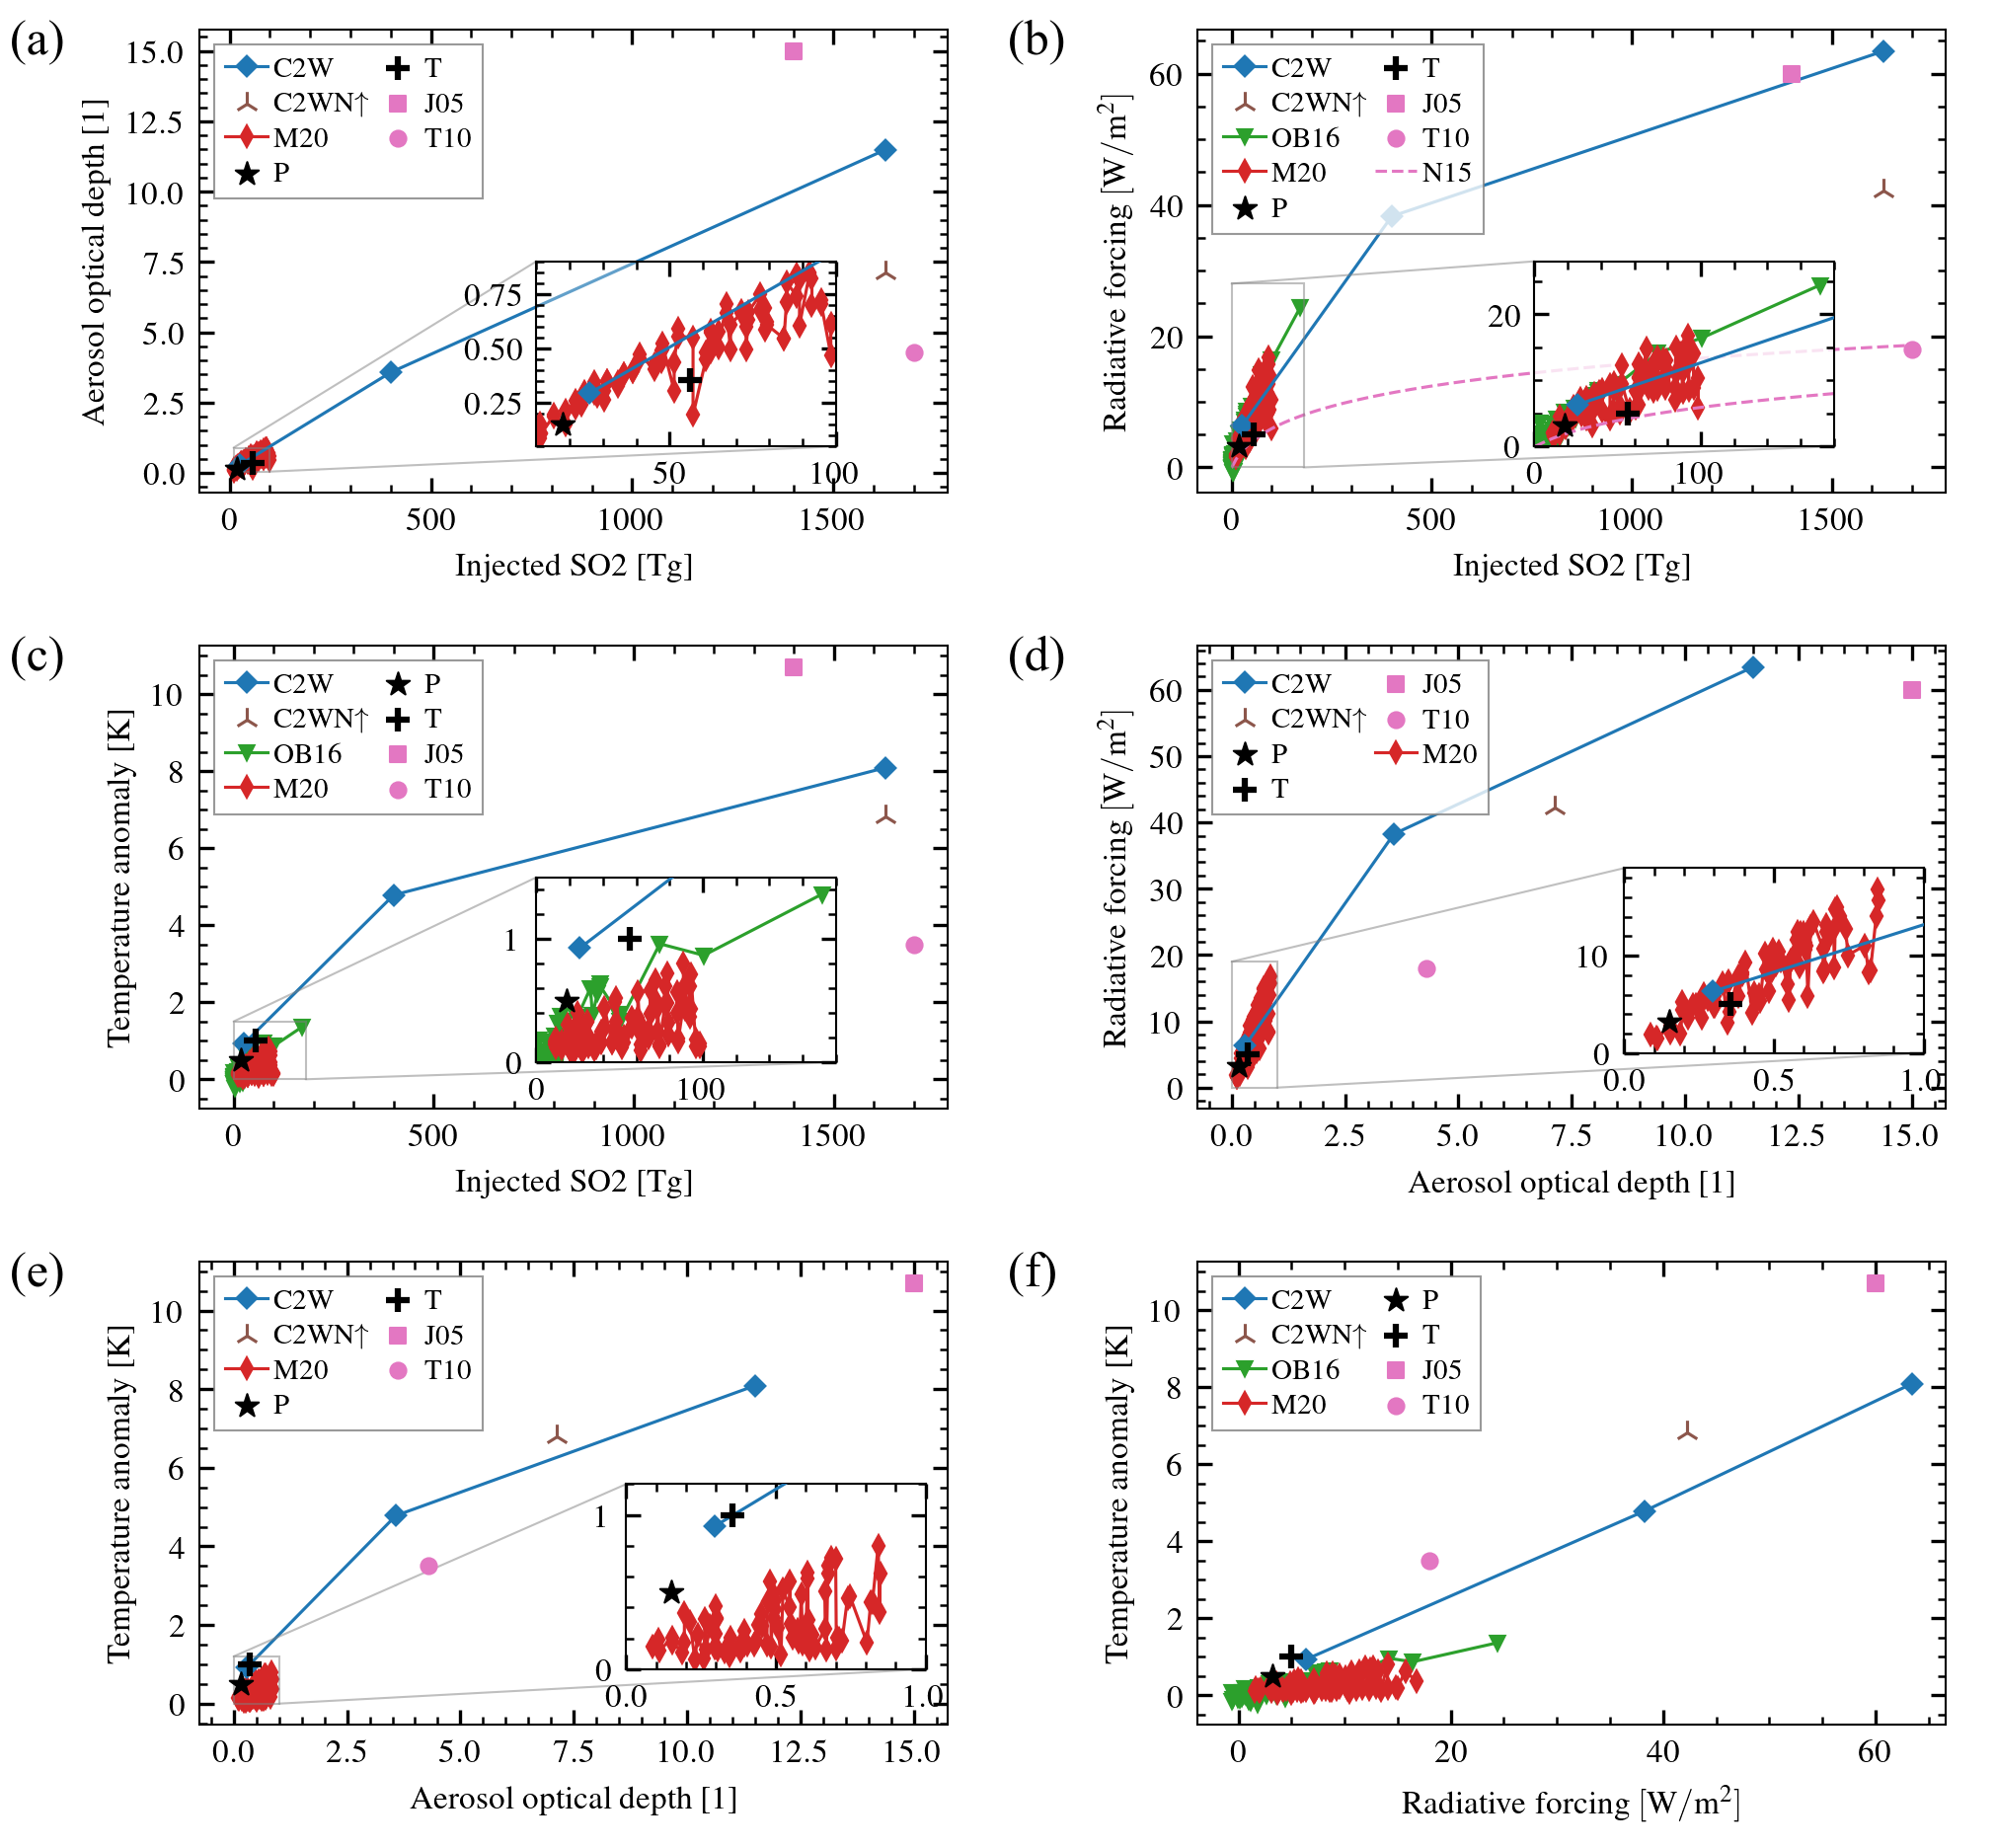
\includegraphics[width=\linewidth]{figures/figure4.png}

  \caption{(a) \gls{aod}, (b) \gls{rf}, and (c) temperature anomaly as a function of
    \iso{}\@. (d) \gls{rf} and (e) temperature anomaly as a function of \gls{aod}. (f)
    Temperature anomaly as a function of \gls{rf}. Blue diamonds labelled \gls{c2w}
    represent tropical cases (\gls{c2wm}, \gls{c2wmp}, \gls{c2ws}), the brown three-branched
    twig signifies the \gls{c2wsn} case, and green downward triangles denote \gls{ob16} data
    from \citet{ottobliesner2016}. The red thin diamonds labelled \gls{m20} display the
    \citet{marshall2020dataset} data. Black star and plus indicate Mt.\ Pinatubo and Mt.\
    Tambora estimates based on observations. The pink square labelled \gls{j05} refers to
    the one-hundred times Mt.\ Pinatubo super-volcano from \citet{jones2005}, and the pink
    disk labelled \gls{t10} represents the \gls{ytt} super-volcano from
    \citet{timmreck2010}. The pink dashed line labelled \gls{n15} is from
    \citet{niemeier2015}, indicating the function in
    Eq.~\ref{eq:niemeier_exponential}.}\label{fig:4_parameter_scan}%
\end{figure*}

% INFO: the conversion between S and SO2 is confirmed by Niemeier and Timmreck (2015)'s
% reference to the Bekki et al. (1996) paper. Bekki uses 6000 Mt SO2, Niemeier uses 3000
% Tg(S).
% NOTAT:
% Kommenter hvordan du går fra rate til konsentrasjon og hvor fornuftig det er.
\citet{niemeier2015} conducted simulations of continuous sulphur injections up to
\(\SI{200}{\tera\gram(\ce{SO2})\mathrm{yr}^{-1}}\) in the ECHAM5's middle atmosphere
version \citep{giorgetta2006} with aerosol microphysics from HAM \citep{stier2005}. They
observed an \gls{rf} dependence on \ce{SO2} injection rate following an inverse
exponential, which converges to \(\SI{-65}{\watt\meter^{-2}}\), depicted in
Fig.~\ref{fig:4_parameter_scan}b as the stippled pink line labelled \gls{n15} and given
as;

\begin{equation}
  \Delta
  R_{\mathrm{TOA}} =
  -\SI{65}{\watt\metre^{-2}}
  \mathrm{e}^{-{\left(\frac{\SI{2246}{\tera\gram(S)yr^{-1}}}{x}\right)}^{0.23}}.
  \label{eq:niemeier_exponential}
\end{equation}
%
Both our simulations and \gls{ob16} exhibit a notably faster increase than this
exponential relationship. The results by \gls{n15}, on which
Eq.~\ref{eq:niemeier_exponential} is based, are all averages over at least three years
of steady sulphur burdens, substantially longer than the time it takes for \gls{rf} to
reach peak values after an eruption. Combined with their lack of a full chemistry model,
a direct comparison between Eq.~\ref{eq:niemeier_exponential} to peak \gls{rf} values
(occurring about one year post-eruption) may not reflect the same chemical and physical
processes. In Eq.~\ref{eq:niemeier_exponential}, \(x\) represents \ce{S}, while the axis
shows values of \ce{SO2}, thus halving of the \ce{SO2} values on the axis gives the
appropriate shape of Eq.~\ref{eq:niemeier_exponential} as a function of \ce{S}.

With these caveats in mind, we observe that \gls{t10}'s results closely align with the
function described in Eq.~\ref{eq:niemeier_exponential}. Starting with an initial input
of \(\SI{850}{\tera\gram(\ce{S})}\) (equivalent to \(\SI{1700}{\tera\gram(\ce{SO2})}\),
representing the \gls{ytt} eruption), their estimated \gls{aod} led to a peak \gls{rf}
of \(\SI{-18}{\watt\meter^{-2}}\), depicted as a pink filled circle in
Fig.~\ref{fig:4_parameter_scan}b. The results from \gls{t10} came from a simulation
using the MPI-ESM climate model, driven by \gls{aod} data from the HAM aerosol model.
This alignment likely stems from the utilization of the same aerosol microphysical model
in both \citet{timmreck2010} and \citet{niemeier2015}, as well as the application of
similar climate models, MPI-ESM and ECHAM5, respectively. The relationship between
climate model families and their implications are further discussed in Appendix C.
Notably, the peak values from \gls{m20} fit well within an upper boundary defined by
\gls{c2w} and \gls{ob16}, and a lower boundary defined by
Eq.~\ref{eq:niemeier_exponential}. Eruptions closer to the equator within \gls{m20}
align with data points near the upper boundary, whereas eruptions at more extreme
latitudes tend to yield weaker peak \gls{rf} values, closer to the lower boundary.
Importantly, none of the eruption simulations exceeded the upper threshold of
\(\SI{-65}{\watt\meter^{-2}}\) as suggested in Eq.~\ref{eq:niemeier_exponential}.

Figure~\ref{fig:4_parameter_scan}c illustrates the response of temperature against
\iso{}. The increase in temperature response with \iso{} decreases for higher \iso{},
showing a similar relationship between \gls{c2w}, \gls{c2wsn}, and \gls{ob16}. Notably,
\gls{t10} and \gls{j05} exhibit respectively much weaker and much stronger temperature
responses to \iso{} than \gls{c2w}. \gls{t10} has a maximum temperature anomaly of only
\(\SI{-3.5}{\kelvin}\) for their \(\SI{1700}{\tera\gram(\ce{SO2})}\) eruption, while
\gls{j05} records a substantially larger maximum temperature anomaly of
\(\SI{-10.7}{\kelvin}\). Since the \gls{m20} experiment was conducted with prescribed
sea-surface temperatures \citep{marshall2020}, preventing the temperature from being
fully perturbed, we do not focus on the \gls{m20} data in the temperature plots but
include them for completeness.

In Fig.~\ref{fig:4_parameter_scan}d, we revisit the relationship between \gls{rf} and
\gls{aod}, focusing on peak values rather than annual and seasonal averages. As
previously discussed, the \gls{rf} to \gls{aod} ratio displays weaker slopes than
previous studies, with the \gls{c2w} peak values not conforming to a linear trend. The
relationship between \gls{rf} and \gls{aod} suggests potential substantial dependencies
on the model and its input parameters, such as latitude, but most notably to an inherent
non-linear \gls{rf} dependence on \gls{aod}. Both the \gls{g16} data in
Fig.~\ref{fig:2_rf_vs_aod_slopes} and the \gls{j05} data originate from the same climate
model. Similarly to what we find from the \gls{c2w} data, the ratio is much stronger for
small eruptions in the industrial era (\gls{g16}) compared to the super-volcano eruption
(\gls{j05}).

In Fig.~\ref{fig:4_parameter_scan}e, we again find that the response of the \gls{c2w}
data decreases with \iso{}, this time in temperature anomaly. Additionally, both the
\gls{c2wsn} and the \gls{j05} cases align well with \gls{c2w}, with the \gls{t10} case
following a similar dependence.

Finally, in Fig.~\ref{fig:4_parameter_scan}f, we compare the temperature and \gls{rf}
responses. Both \gls{c2w} and \gls{ob16} show a near-linear relationship between
temperature and \gls{rf}. The \gls{c2w} data indicate a steeper slope, implying stronger
temperature perturbations as compared to \gls{ob16}. However, potential biases exist in
the values from the analysis of \gls{ob16}, as outlined in Appendix B,
section~\ref{ap:ob16}. This, along with considerable noise, results in the analysis of
\gls{ob16} temperature anomalies being less reliable. As in
Fig.~\ref{fig:4_parameter_scan}e, the \gls{c2wsn} case along with both the \gls{t10} and
\gls{j05} cases closely follow the temperature to \gls{rf} dependence of \gls{c2w}.

The almost linear relationship between \gls{aod} and \iso{} for the \gls{c2w} data in
Fig.~\ref{fig:4_parameter_scan}a suggests a comparable trend for \gls{rf} versus \iso{}
in Fig.~\ref{fig:4_parameter_scan}b, as seen for \gls{rf} versus \gls{aod} in
Fig.~\ref{fig:4_parameter_scan}d. For the same reason, we expect
Fig.~\ref{fig:4_parameter_scan}e to show a similar pattern for \gls{c2w} as observed in
Fig.~\ref{fig:4_parameter_scan}c.

This relationship, along with the functional relationships between all other parameters
shown in Fig.~\ref{fig:4_parameter_scan}, are illustrated in
Fig.~\ref{fig:5_diagram_of_function_relations}. There, we show that from assuming a
linear dependency of \gls{aod} on \iso{} (\(ax+b\)), and of temperature on \gls{rf}
(\(cx+d\)), we must have that \(f\), \(g\), \(h\), and \(k\) all have the same
functional form, where \(f: \ce{SO2} \to \mathrm{RF}\), \(g: \mathrm{AOD} \to
\mathrm{T}\), \(h: \ce{SO2} \to \mathrm{T}\), and \(k: \mathrm{AOD} \to \mathrm{RF}\).
From this, we deduce that \(f(x)=k(ax+b)\) and \(h(x)=f(cx+d)=g(ax+b)\), and finally
that \(h(x)=k(acx+ad+b)\), concluding that \(f\), \(g\), \(h\), and \(k\) have the same
functional form.

\begin{figure}
  \centering

  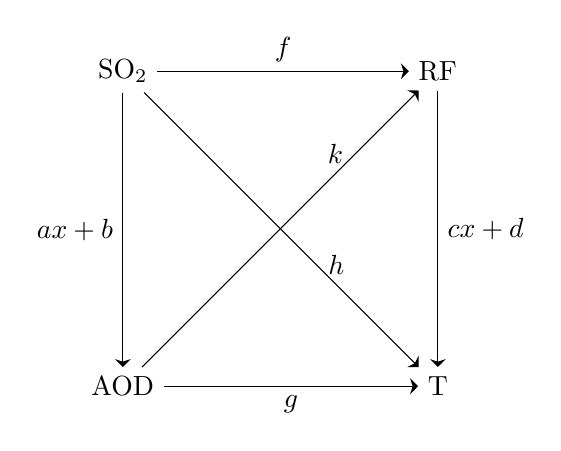
\begin{tikzpicture}[>={Stealth[length=1mm,width=2mm]}]
    % Place the letters in the corners
    \node (A) at (0,0) {AOD}; \node (T) at (4,0) {T}; \node (RF) at (4,4) {RF}; \node (S) at
    (0,4) {\ce{SO2}};
    % Draw arrows between the letters
    \draw[->] (A) -- node[midway, below] {\(g\)} (T); \draw[->] (RF) -- node[midway, right]
    {\(cx+d\)} (T); \draw[->] (S) -- node[midway, above] {\(f\)} (RF); \draw[->] (S) --
    node[midway, left] {\(ax+b\)} (A); \draw[->] (S) -- node[pos=0.7, above] {\(h\)} (T);
    \draw[->] (A) -- node[pos=0.7, above] {\(k\)} (RF);
  \end{tikzpicture}

  \caption{Diagram describing the functional relationships of the parameters shown in
    Fig.~\ref{fig:4_parameter_scan}.}\label{fig:5_diagram_of_function_relations}%
\end{figure}

\subsection{Climate sensitivity estimate}

As previously mentioned, \gls{j05} is similar to \gls{c2ws} concerning \gls{rf} values,
yet differ in both \gls{aod} and temperature. To investigate this discrepancy, we here
conduct a comparison between their climate feedback parameter \(\alpha\) (where
\(s=1/\alpha\) is the climate sensitivity parameter) with our climate resistance,
denoted as \(\rho\), and the \gls{tcrp} \(1/\rho\) (where
\(\mathrm{TCS}=F_{2\times\ce{CO2}}\times \mathrm{TCRP}\) is the transient climate
sensitivity and \(F_{2\times\ce{CO2}}\) is the forcing due to a doubling of
pre-industrial \ce{CO2} concentration). As the forcing of volcanic eruptions typically
lasts for about a year, a duration too brief for the timescales at which \(F=\rho T\)
remains valid, an alternative approach involves using a time-integral form introduced by
\citet{merlis2014}:

\begin{equation}
  \int_0^{\tau}F \mathrm{d}t=\rho\int_{0}^{\tau}T \mathrm{d}t
  \label{eq:climate-resistance-orig}
\end{equation}
\begin{equation}
  \rho=\frac{\int_0^{\tau}F \mathrm{d}t}{\int_{0}^{\tau}T \mathrm{d}t}.
  \label{eq:climate-resistance}
\end{equation}

If the upper bound of the integral, \(\tau\), is sufficiently large, so that the upper
ocean heat content is the same at \(t=0\) and \(t=\tau\), this approach agrees with
\(F=\rho T\) for long-term forcing \citep{gregory2016} (\citet{merlis2014} used \(\tau
=\SI{15}{\mathrm{yr}}\)). Additionally, we note that the climate resistance and the
climate feedback parameter are associated with the ocean heat uptake efficiency
(\(\kappa\)) through \(\rho =\alpha +\kappa\) \citep{gregory2016}.

The climate feedback parameter estimated by \citet{jones2005} is \(\alpha \simeq
\SI{4}{\watt\metre^{-2}\kelvin^{-1}}\), exceeding twice the value obtained by
\citet{gregory2016} in their simulations of Mt.\ Pinatubo using the same HadCM3 climate
model. We determine the climate resistance using the integral-form computation outlined
in Eq.~\ref{eq:climate-resistance} and adopting \(\tau =\SI{20}{\mathrm{yr}}\). The
estimated climate resistance from the three tropical simulation cases (with four in each
ensemble) converges to \(\rho =\SI{2.5(4)}{\watt\metre^{-2}\kelvin^{-1}}\), and
\gls{tcrp} values of \(1/\rho=\SI{0.41(5)}{\kelvin\watt^{-1}\metre^{2}}\), as reported
in table~\ref{tab:trcp}, and is therefore assumed to be a good estimate of \(\alpha\).

Importantly, our estimate agrees well with \gls{g16}, while the \gls{j05} estimate of
\(\alpha \simeq \SI{4}{\watt\metre^{-2}\kelvin^{-1}}\) is still notably higher than
both. Since the temperature perturbation obtained by \gls{j05} was higher than any of
our \gls{cesm2} cases, it indicates that the forcing used by \gls{j05} must be stronger.
The peak value of the \gls{j05} \gls{rf} is similar to the \gls{c2ws} case, and as such,
the overall stronger forcing must originate from the development of the forcing time
series rather than the peak value.

\begin{table}
  \centering

  \caption{Estimated climate resistance and \gls{tcrp} by use of the method outlined by
    \citet{merlis2014}. Estimates are based on ensembles with four members and \(\tau
    =\SI{20}{\mathrm{yr}}\) using Eq.~\ref{eq:climate-resistance}.}\label{tab:trcp}%
  \begin{tabular}{ccc}
    Simulation  & \(\rho [\si{\watt\metre^{-2}\kelvin^{-1}}]\) & \(1/\rho\)        \\
    \gls{c2ws}  & \(\num{2.21(5)}\)                            & \(\num{0.45(1)}\) \\
    \gls{c2wmp} & \(\num{2.51(6)}\)                            & \(\num{0.40(1)}\) \\
    \gls{c2wm}  & \(\num{2.9(6)}\)                             & \(\num{0.36(7)}\) \\
    Total       & \(\num{2.5(4)}\)                             & \(\num{0.41(5)}\) \\
  \end{tabular}
\end{table}

\section{Discussion}\label{sec:discussion}

% NOTE: Suggested layout for the
% Discussion:
% - Explain the results and emphasize significant findings clearly
% - Discuss the impact and importance of results compared with recent relevant research
% Conclusion
% - The justification for these objectives: Why is the work important?
% - Summarize the key points made in the other sections
% - Conclude overall discussion of article
% - Link this section to the introduction

% RF / AOD linearity does not hold for large eruptions
Figures~\ref{fig:2_rf_vs_aod_slopes},~\ref{fig:3_rf_to_aod_ratios}, and
\ref{fig:4_parameter_scan}d demonstrate that as the \gls{aod} exceeds approximately
\(1.0\), the linear \gls{rf} dependence of approximately
\(\SI{-20}{\watt\metre^{-2}\mathrm{AOD}^{-1}}\) no longer holds. The sublinear increase
in \gls{rf} with \iso{} in Fig.~\ref{fig:4_parameter_scan}b for large eruptions is
consistent with previous results from simulations using similar climate models of
smaller historic eruptions (\gls{g16}) and of super-volcanoes (\gls{j05}). Such a change
in ratio has been attributed to larger eruptions, injecting more \ce{SO2}, leading to
larger aerosols, and hence less effective radiation scattering, thereby reducing the
\gls{rf} for the same \iso{} \citep{english2013, timmreck2010, timmreck2018}.

% Latitude is more important for the development of the RF / AOD ratio
The non-linear relationship between peak \gls{rf} and \gls{aod} values is a strong
signature in both Figs.~\ref{fig:2_rf_vs_aod_slopes} and~\ref{fig:3_rf_to_aod_ratios}.
Across eruptions of the same strength, the ratio stays relatively constant, leading to a
close to \(\SI{-10}{\watt\metre^{-2}\mathrm{AOD}^{-1}}\) slope for \gls{c2wmp} and a
\(\SI{-5}{\watt\metre^{-2}\mathrm{AOD}^{-1}}\) slope for \gls{c2ws}. Still, a non-linear
development in the \gls{rf} to \gls{aod} ratio is found, most notably across all
tropical eruptions. Similar to the results of \citet{marshall2020}, we find in
\gls{c2wmp} and \gls{c2ws} that the post-peak period (second and third post-eruption
years) has a stronger aerosol forcing efficiency compared to the pre-peak period (first
post-eruption year). The post-peak period of \gls{c2wm} is elevated as compared to the
pre-peak period, resulting in a decreasing aerosol forcing efficiency from the first to
the second and third post-eruption years, in contrast to the other tropical eruptions.

Focusing on the pre-peak period, we find tropical eruptions to differ from eruptions at
high latitudes. During the pre-peak period, all tropical eruptions show a decreasing
aerosol forcing efficiency, while no significant change in the \gls{rf} to \gls{aod}
ratio is found from the \gls{c2wsn} case. The full \gls{m20} dataset indicates an
increasing aerosol forcing efficiency also during the pre-peak period, contrasting the
decreasing efficiency found from their tropical eruptions and supporting the latitudinal
dependence we find in \gls{c2wsn}. While we find a linear relationship to be a useful
approximation of \gls{rf} dependence on \gls{aod} for eruptions similar to or smaller
than Mt.\ Pinatubo, additional factors must be considered for larger eruptions.
% NOTAT:
% Reformuler så du fokuserer på hvordan resultatene avviker fra linearitet. Så kan du ta faktorene som en mulig forklaring, men bør sitere. Spesielt reflectance og gravitational pull har du ikke nevnt før?
These factors, such as \ce{OH} scarcity and aerosol growth, influence reflectance and
their gravitational pull, substantially impacting both \gls{aod} and \gls{rf} evolution,
as highlighted by \citet{timmreck2010}. The large difference in ratio found when
comparing eruption magnitudes suggests that \iso{} is crucial when estimating the
time-average of the \gls{rf} to \gls{aod} ratio. However, latitude and, in particular,
aerosol dispersion are more influential in determining the post-eruption evolution of
the ratio, particularly during the pre-peak period.

% Models vary in their SO2 to H2SO4 chemistry/physics, but are comparatively consistent in representing AOD, RF and temperature.
The biggest spread in the data shown in Fig.~\ref{fig:4_parameter_scan} is found when
relating \iso{} to any of the three output parameters. As the amount of \iso{}
increases, both \gls{aod}, \gls{rf}, and temperature across models have a big spread.
The \gls{aod} to \iso{} relationship is consistent within similar models, even when
comparing simulations of volcanic eruptions \citep{timmreck2010} and continuous
injection of \ce{SO2} \citep{niemeier2015}, but has a wide spread at high values of
\iso{} across model families (Figs.~\ref{fig:4_parameter_scan}a,b,c). Comparatively, the
\gls{rf} (Fig.~\ref{fig:4_parameter_scan}d) and temperature
(Fig.~\ref{fig:4_parameter_scan}e) as a function of \gls{aod}, as well as temperature as
a function of \gls{rf} (Fig.~\ref{fig:4_parameter_scan}f), demonstrate a smaller spread
across models. \citet{marshall2019, marshall2020, marshall2021} use a code with seven
log-normal modes to simulate aerosol mass and number concentrations, along with an
atmosphere-only configuration of the UM-UKCA with prescribed sea-surface temperatures
and sea-ice extent \citep{marshall2019}. This approach is in contrast with \gls{cesm2},
operating as an \gls{esm}, but with a simpler aerosol chemistry model in the \gls{mam3}.
The family of models to which \gls{m20} is based is different from that of \gls{c2w} and
\gls{ob16}, and also different from the \gls{t10} and \gls{n15}, as described in
Appendix C. Based on Fig.~\ref{fig:4_parameter_scan}, we find the model family to be
pivotal in determining the estimated \gls{aod} and \gls{rf} magnitudes from \iso{},
whereas the various models generally demonstrate more consistency in representing
\gls{rf} from \gls{aod}. Despite the large spread in \iso{} and corresponding response
in \gls{rf}, none of the eruption simulations shown in Fig.~\ref{fig:4_parameter_scan}
violated the suggested upper threshold of \(\SI{-65}{\watt\metre^{-2}}\) as defined in
Eq.~\ref{eq:niemeier_exponential}.

% AOD time series are different across eruption magnitudes, and peak at later times
\citet{timmreck2010} highlights that for sufficiently large eruptions, \ce{OH} radicals
are too scarce, which limits \ce{SO2} oxidation. The \gls{aod} peak in the \gls{ytt}
simulation of \gls{t10} occurs six months after Mt.\ Pinatubo's peak. This aligns with
our results, as illustrated in Fig.~\ref{fig:1_compare_waveform}a, where \gls{c2wm}
shows an earlier \gls{aod} peak compared to \gls{c2wmp} and \gls{c2ws}. While the peak
\gls{rf} value of \gls{t10} occurs \(7\)--\(8\) months post-eruption, similar to
\gls{c2w}, the \gls{j05} peak anomaly occurs one year post-eruption. Additionally, as
\citet{jones2005} obtains a climate feedback parameter larger than both what
\citet{gregory2016} found for the same climate model and larger than the climate
resistance obtained here from \gls{c2w}, we conclude that such a simple approach of
scaling the \gls{aod} of smaller eruptions to represent larger eruptions is
insufficient. Moreover, having a small ensemble of large eruptions to represent smaller
eruptions is also insufficient when simulating from \iso{}, as both \gls{aod} and
temperature evolution are found to develop differently.

\section{Summary and conclusions}\label{sec:conclusions}

We consider three medium to super-volcano sized eruptions and compare them to previously
reported results. We find the commonly adopted \gls{rf} dependence on \gls{aod} of
\(\sim\SI{-20}{\watt\metre^{-2}\mathrm{AOD}^{-1}}\) to be representative for Mt.\
Pinatubo-sized eruptions. Larger eruptions, with one to two orders of magnitude larger
injections of \ce{SO2}, are found to have an \gls{rf} dependence on \gls{aod} closer to
\(\sim\SI{-10}{\watt\metre^{-2}\mathrm{AOD}^{-1}}\) and
\(\sim\SI{-5}{\watt\metre^{-2}\mathrm{AOD}^{-1}}\). A shallower slope for larger
eruptions is also consistent with peak values from previous studies of super-volcanoes.

The time-after-eruption dependence of the ratio between \gls{rf} and \gls{aod} is found
to weaken with time, resulting in a decreasing aerosol forcing efficiency in the
pre-peak period. The effect is found across all eruption sizes, but only the tropical
cases show a clear trend. The high-latitude case displays an almost constant efficiency
with time. These results agree with a reanalysis of the tropical data in
\citet{marshall2020dataset}. Thus, these findings provide strong supporting evidence
that latitude is generally significant in determining the aerosol forcing efficiency,
particularly as a function of time-after-eruption. These findings emphasise the
complexity of volcanic impacts on climate, demonstrating significant differences in
climatic response depending on eruption magnitude and latitude.

We find that the \gls{aod} peak arrives later for larger eruptions than for smaller
ones, and also that larger eruptions produce a sharper peak in the \gls{aod} time
series. The \gls{rf} time series are similar across all eruption sizes, and while the
smallest eruption experiences a faster temperature decay, the two larger eruptions
produce time series indistinguishable in development for both \gls{rf} and temperature.
Thus, a simple scaling of the \gls{aod} or temperature time series from a smaller
eruption is insufficient in representing that of larger volcanic eruptions.

% NOTAT:
% Du kan godt diskutere hvordan modellfamilie ser ut til å bestemme en god del av variasjonen, men plaser future work i konklusjonene
% NOTAT:
% Reformuler dette som en forskjell mellom modellfamilier, og poengter forskjellene det gir seg utslag i.
Considering \iso{} and the peak values of \gls{aod} and \gls{rf}, a large spread is
found across model families in Fig.~\ref{fig:4_parameter_scan}. Improving the
consistency between model families in how the chemistry and physics of \ce{SO2} and
\ce{H2SO4} are represented is an important step in enhancing the accuracy of simulated
volcanic eruptions' influence on climate by models.
% NOTAT:
% Jeg ser ikke helt hva dette henspeiler på? Er det i sammenheng med flere modeller (over?)
% NOTAT:
% Jeg foreslår at du reformulerer dette som å studere sammenhengen mellom enkeltutbrudd og kontinuerlige utslipp
Simulations of larger volcanic eruptions with \iso{} greater than
\(\SI{200}{\tera\gram(\mathrm{SO2})}\) would provide useful information for a more
precise determination of the \gls{rf} to \gls{aod} ratio in the non-linear regime. This
would also serve as a useful test to check if a comparison between \ce{SO2} injection
events and continuous \ce{SO2} injection is reasonable. Introducing a spread in latitude
similar to the \citet{marshall2020dataset} dataset would allow for better comparison
between eruptions across all latitudes and the suggested lower limit following
Eq.~\ref{eq:niemeier_exponential}, describing a situation of aerosol saturation.

% NOTAT:
% Bruk mer tid på konklusjonene fra fig 4 her. Lineære sammenhenger, mulig RF max på -65 W/m^2 etc.
We find that the suggested upper threshold from Eq.~\ref{eq:niemeier_exponential} is not
violated by any eruption simulation. Thus, even larger volcanic eruption simulations
injecting \(\SI{3000}{\tera\gram(\mathrm{SO_2})}\) or more would provide insight about
whether the linearity holds in Fig.~\ref{fig:4_parameter_scan}f, such that either the
temperature anomaly also reaches a limit or the \(\SI{-65}{\watt\metre^{-2}}\) limit is
exceeded, or non-linearities appear in the temperature to \gls{rf} relationship.

\clearpage
%%%%%%%%%%%%%%%%%%%%%%%%%%%%%%%%%%%%%%%%%%%%%%%%%%%%%%%%%%%%%%%%%%%%%
% ACKNOWLEDGMENTS
%%%%%%%%%%%%%%%%%%%%%%%%%%%%%%%%%%%%%%%%%%%%%%%%%%%%%%%%%%%%%%%%%%%%%
\acknowledgments{}
%  Keep acknowledgments (note correct spelling: no ``e'' between the ``g'' and
% ``m'') as brief as possible. In general, acknowledge only direct help in
%  writing or research. Financial support (e.g., grant numbers) for the work done,
%  for an author, or for the laboratory where the work was performed must be
%  acknowledged here rather than as footnotes to the title or to an author's name.
%  Contribution numbers (if the work has been published by the author's institution
%  or organization) should be placed in the acknowledgments rather than as
%  footnotes to the title or to an author's name.

% https://www.sigma2.no/acknowledgements
The simulations were performed on resources provided by Sigma2 --- the National
Infrastructure for High Performance Computing and Data Storage in Norway.

This work was supported by the Tromsø Research Foundation under Grant Number 19\_SG\_AT.

Thanks to both Maria Rugenstein and Martin Rypdal for valuable discussions. We would
also like to thank the authors of \citet{gregory2016, ottobliesner2016,
  marshall2020dataset} for making their data available.

%%%%%%%%%%%%%%%%%%%%%%%%%%%%%%%%%%%%%%%%%%%%%%%%%%%%%%%%%%%%%%%%%%%%%
% DATA AVAILABILITY STATEMENT
%%%%%%%%%%%%%%%%%%%%%%%%%%%%%%%%%%%%%%%%%%%%%%%%%%%%%%%%%%%%%%%%%%%%%
%
%
\datastatement{}
%  The data availability statement is where authors should describe how the data underlying
%  the findings within the article can be accessed and reused. Authors should attempt to
%  provide unrestricted access to all data and materials underlying reported findings.
%  If data access is restricted, authors must mention this in the statement. See
%  {http://www.ametsoc.org/PubsDataPolicy} for more info.

% FIXME: NRIS archive DOI
% https://documentation.sigma2.no/nird_archive/user-guide.html
Data generated directly from output fields of \gls{cesm2} are available at \emph{refer
  to Sigma2 archive}, and were generated using scripts available at
\url{https://github.com/engeir/cesm-data-aggregator}. Analysis scripts are available at
\url{https://github.com/engeir/paper1-code} and is published to
\url{https://zenodo.org/doi/10.5281/zenodo.10229427}. Source code used to generate
\gls{cesm2} input files are available at
\url{https://github.com/engeir/cesm2-volcano-setup}.

%%%%%%%%%%%%%%%%%%%%%%%%%%%%%%%%%%%%%%%%%%%%%%%%%%%%%%%%%%%%%%%%%%%%%
% APPENDIXES
% https://www.ametsoc.org/index.cfm/ams/publications/author-information/latex-author-info/documentation-for-ams-latex-template1/
%%%%%%%%%%%%%%%%%%%%%%%%%%%%%%%%%%%%%%%%%%%%%%%%%%%%%%%%%%%%%%%%%%%%%
%
%% If only one appendix, use

%\appendix

%% If more than one appendix, use \appendix[<letter>], e.g.,

%\appendix[A]

%% Appendix title is necessary! For appendix title:

%\appendixtitle{Title of Appendix}

%%% Appendix section numbering (note, skip \section and begin with \subsection)
%
% \subsection{First primary heading}

% \subsubsection{First secondary heading}

% \paragraph{First tertiary heading}

\appendix

\appendix[A]

\appendixtitle{Simulation set up and output}

Input files used in the simulations were created by modifying the file available at
\url{http://svn.code.sf.net/p/codescripts/code/trunk/ncl/emission/createVolcEruptV3.ncl},
using a Python package available on GitHub at
\url{https://github.com/engeir/volcano-cooking} or through the Python Package Index
(PyPI). The package is available both as a library and a Command Line Interface (CLI),
and is used to create volcanic eruptions with a specified amount of \ce{SO2} that is
injected over six hours at a given latitude, longitude, and altitude. All volcanic
\ce{SO2} files are created from a shell script by setting the eruption details in a JSON
file that is read by the \texttt{volcano-cooking} CLI at a fixed version, ensuring a
reproducible experiment setup.

We are using the coupled model version \texttt{BWma1850} component setup to run the
\gls{cesm2}, and an accompanying fixed sea-surface temperature version,
\texttt{fSST1850}, to obtain estimates of the \gls{rf}. The applied \texttt{fSST1850} is
not from a standardised component setup but is instead explicitly
specified.\footnote{\fssturl} The component setup \texttt{BWma1850} and
\texttt{fSST1850} differ in that the latter uses a prescribed sea-ice (\texttt{CICE ->
  CICE\%PRES}), a prescribed data ocean (\texttt{POP2\%ECO\%DEP -> DOCN\%DOM}) and a stub
wave component instead of the full \gls{ww3} (\texttt{WW3 -> SWAV}).

The important input data used in the model simulations are \iso{} in units of teragrams
(\(\si{\tera\gram(\ce{SO2})}\)), used to simulate volcanic eruptions. \gls{rf} is
calculated as the combined (\gls{sw} and \gls{lw}) all-sky \gls{toa} energy imbalance,
where the \gls{cesm2} provide the output variables \gls{fsnt} and \gls{flnt}. Thus,
\(\mathrm{RF_*}= \mathrm{FSNT} - \mathrm{FLNT}\), and taking the difference between
volcanic forcing simulations and a control simulation gives the final estimate of
\gls{rf} (\(\mathrm{RF}=\mathrm{RF_{VOLC}}-\mathrm{RF_{CONTROL}}\))
\citep{marshall2020}. The \gls{rf} calculation is based on \texttt{fSST1850}, hence this
outline specifically describes how to calculate \gls{erf} as opposed to \gls{irf}, which
instead is the difference between the \gls{erf} and the sum of all rapid atmospheric
adjustments \citep{marshall2020,smith2018}. The \gls{aod} is obtained from the output
variable \gls{aodm}, while global temperature is saved by \gls{cesm2} to the variable
\gls{trefht}. The analysis of this work is performed using these four variables.

During analysis, one outlier was found in the ensemble representing \gls{c2wm},
specifically in the temperature time series. This ensemble member was the February 15,
1850, eruption, which was changed in favor of a February 15, 1851, eruption in the
\gls{c2wm}, \gls{c2wmp}, and \gls{c2ws} ensembles. For completeness, the February 15,
1850, eruption is still included in the online archive.

\appendix[B]

\appendixtitle{External data}

\subsection{Otto-Bliesner data analysis}\label{ap:ob16}

Data from \citet{ottobliesner2016} are the original input data of \iso{} as used in
their model simulations, along with \gls{rf} and temperature output data. The \iso{} can
be downloaded with a direct link from
\url{https://svn-ccsm-inputdata.cgd.ucar.edu/trunk/inputdata/atm/cam/volc/IVI2LoadingLatHeight501-2000_L18_c20100518.nc},
or found at \url{https://www.cesm.ucar.edu/working-groups/paleo/simulations/ccsm4-lm}
and \url{https://svn-ccsm-inputdata.cgd.ucar.edu/trunk/inputdata/atm/cam/volc/}. Only
the peak values of the \ce{SO2} dataset were used in the analysis. Output variables are
available at
\url{https://www.earthsystemgrid.org/dataset/ucar.cgd.cesm2le.atm.proc.daily_ave.html}.

Since the \gls{ob16} dataset contains a five-member ensemble, the final \gls{rf} and
temperature time series used were ensemble means. A single control simulation time
series is used to remove seasonal dependence from the temperature, where the control
simulation is averaged into a climatology mean. Further, a drift in the temperature is
removed by subtracting a linear regression fit. \gls{rf} has seasonality removed in the
Fourier domain.

The time of an eruption is found based on a best attempt at aligning the \ce{SO2} time
series with both the \gls{rf} time series and the temperature time series. The \gls{rf}
and temperature peak values are taken as the value of the time series at the time of an
eruption according to the \ce{SO2} time series. Missing the true peak means the found
peaks will be biased towards lower values. However, instances where eruptions occur
close in time will contribute a bias to higher values. These biases contribute to a
greater uncertainty related to \gls{ob16} in Figs.~\ref{fig:4_parameter_scan}b,c,f.

\subsection{Marshall data analysis}\label{ap:m20}

Data used to compute the \gls{m20} values were from \citet{marshall2020dataset},
available at \url{https://doi.org/10.5285/232164e8b1444978a41f2acf8bbbfe91}. As each
file includes a single eruption, peak values of \gls{aod}, \gls{rf}, and temperature
were found by applying a Savitzky-Golay filter of third order and one-year window
length, and choosing the maximum value \citep{savitzky1964}.

\subsection{Gregory data analysis}\label{ap:g16}

Data used to compute \gls{g16} values were kindly provided by Jonathan Gregory (personal
communication). The full 160-year-long time series were further analysed by computing
annual means.

\appendix[C]

\appendixtitle{Model families}

The model used here was the \gls{cesm2} with the \gls{waccm} atmosphere in the \gls{ma}
configuration. The \gls{ma} configuration uses the \gls{mam3} \citep{gettleman2019}, a
simplified and computationally efficient default setting within the \gls{cam5}
\citep{liu2016}, as described in \citet{liu2012}. The \gls{mam3} was developed from
MAM7, consisting of the seven modes Aitken, accumulation, primary carbon, fine dust,
fine sea salt, coarse dust, and coarse sea salt. Instantaneous internal mixing of
primary carbonaceous aerosols with secondary aerosols and instantaneous ageing of
primary carbonaceous particles are assumed by emitting primary carbon in the
accumulation mode \citep{liu2016}. As dust absorbs water efficiently and is expected to
be removed by wet deposition similarly to sea salt, fine dust is merged with fine sea
salt into the accumulation mode and coarse dust is merged with coarse sea salt into a
coarse mode. The coarse mode will quickly revert to its background state below the
tropopause \citep{liu2012}. Consequently, \gls{mam3} features the three modes Aitken,
accumulation, and coarse \citep{liu2016}.

The \gls{cesm2} is an ancestor of \gls{cesm1} used by \gls{ob16}. They belong to a
different model family than both the HadCM3 (\gls{j05} and \gls{g16}) and the UM-UKCA
(\gls{m20}), which is an extended version of HadGEM3 \citep{dhomse2014}, and an ancestor
of HadCM3. A third model family is represented through ECHAM5 (\gls{n15}) and MPI-ESM
(\gls{t10}), where the latter is related to the former via the ECHAM6. A summary of the
model code genealogy is in table~\ref{tab:model-family}, based on the model code
genealogy map created by \citet{kuma2023}.

\begin{table*}
  \centering
  \caption{Overview of various model codes grouped into families according to the model
    code genealogy map by \citet{kuma2023}, with each table entry also indicating the
    specific model code used in the referenced papers of this
    study.}\label{tab:model-family}

  \begin{tabular}{ccc}
    Family relation                                                         & Model name           & Data name  \\
    \multirow{2}{*}{CESM1 \(\rightarrow\) CESM1-CAM5 \(\rightarrow\) CESM2} & CESM1                & \gls{ob16} \\
                                                                            & CESM2
                                                                            & \emph{This
    contribution}                                                                                               \\
    \rowcolor{LightGray}                                                    & HadCM3
                                                                            & \gls{j05}, \gls{g16}              \\
    \rowcolor{LightGray}\multirow{-2}{*}{\shortstack{HadCM3 \(\rightarrow\) HadGEM1
    \(\rightarrow\)                                                                                             \\
    HadGEM2 \(\rightarrow\) HadGEM3 \(\rightarrow\) UM-UKCA}}               & UM-UKCA              &
    \gls{m20}                                                                                                   \\
    \multirow{2}{*}{ECHAM5 \(\rightarrow\) ECHAM6 \(\rightarrow\) MPI-ESM}  & ECHAM5               &
    \gls{n15}                                                                                                   \\
                                                                            & MPI-ESM              & \gls{t10}  \\
  \end{tabular}
\end{table*}

%%%%%%%%%%%%%%%%%%%%%%%%%%%%%%%%%%%%%%%%%%%%%%%%%%%%%%%%%%%%%%%%%%%%%
% REFERENCES
%%%%%%%%%%%%%%%%%%%%%%%%%%%%%%%%%%%%%%%%%%%%%%%%%%%%%%%%%%%%%%%%%%%%%
% Make your BibTeX bibliography by using these commands:
% \bibliographystyle{ametsocV6}
% \bibliography{references}

\bibliographystyle{ametsocV6}

% \bibliography{~/science/ref/ref}

\bibliography{references}

\clearpage

\printglossary[type=\acronymtype,title=List of Acronyms]

\end{document}
